\documentclass[12pt,notitlepage]{report}
\pagestyle{plain}

\usepackage[utf8]{inputenc}
\usepackage[czech,slovak,english]{babel}

\usepackage{a4wide}
\usepackage[left=4cm,right=2.5cm,top=2.5cm,bottom=2.5cm]{geometry}
\usepackage{setspace}

\usepackage{amsmath}
\usepackage{amsfonts}
\usepackage{amssymb}
\usepackage{amsthm}

\usepackage{float}
\usepackage[pdftex]{graphicx}
\usepackage{epstopdf}

\usepackage{booktabs}
\usepackage{multirow}
\usepackage{courier}

\usepackage{listings}
\lstset{language=c++, basicstyle=\ttfamily\footnotesize}
\usepackage{algorithmic}
\usepackage{algorithm}

% Now, switch on what is appropriate for czech:

% czech quotation marks
% \bq - begin quotation, \eq - end quotation
\def\bq{\mbox{\kern.1ex\protect\raisebox{-1.3ex}[0pt][0pt]{''}\kern-.1ex}}
\def\eq{\mbox{\kern-.1ex``\kern.1ex}}
%\setlanguage{\czech}

{%                                      % Begin a group for which " is active
\catcode`\"=\active                     % Make " an active character
\catcode`\@=11                          % Make @ an active character
%
%  \csdoublequoteson
%
%       This macro makes " an active character, resets the control sequence
%       \dblqu@te to L (left), and defines \dq as a replacement for ".
%
\gdef\csdoublequoteson{%                % \csdoublequoteson enables "
    \gdef"{\czechquotes}%               % Define " as \czechquotes
    \global\catcode`\"=\active%         % Make " an active character
    \global\chardef\dq=`\"%             % Double-quote char. via \dq
    \global\let\dblqu@te=L%             % Always start with a left double-quote
    }                                   % End of macro
%
%  \bq, \eq
%
%      These macros define default characters for czech left and right
%      double quotes. Czech opening quote is created from two commas with
%      kerning depending on fontdimen four parameter of current font.
%      Better solution should be specially designed character with
%      proper kernings; if you have such characters in fonts
%      (e.g. in DC-fonts), use it instead. (e.g. define
%      macros \bq and \eq e.g. \def\bq{\char"130 }
%      in your document/style file-- not in csquote.sty!)
%      Similar solution is used for czech right quote.
%
%      \cs existence test, stolen from TeXbook exercise 7.7
\def\ifundefined#1{\expandafter\ifx\csname#1\endcsname\relax }%
%
%      another macro to be more efficient in time and space
\global\chardef\f@@r=4
%
\ifundefined{bq}%
\gdef\bq{\kern-.25\fontdimen\f@@r\font,\kern-.8\fontdimen\f@@r\font,%
                \kern-.35\fontdimen\f@@r\font}%
\fi
\ifundefined{eq}%
\gdef\eq{\kern-.35\fontdimen\f@@r\font`\kern-.8\fontdimen\f@@r\font`%
                \kern-.25\fontdimen\f@@r\font}
\fi
%
% Macro \uv for other usage of \bq and \eq.
%
\ifundefined{uv}%
        \gdef\uv#1{\bq #1\eq}
\fi
%
% \testquotes macro gives warning if citation span this place
%
\gdef\testquotes{\if R\dblqu@te
        \message{Warning: You forgot right double quote!}%
        \let\dblqu@te=L\fi}
%
%  Define the macro that will be executed whenever " is encountered.
%
\gdef\czechquotes{\protect\czechqu@tes}
\gdef\czechqu@tes{%
        %  If the double-quote is the first character in a new paragraph,
        %  make sure it becomes a left double-quote.  This case can be
        %  detected by checking to see if TeX is currently in vertical mode.
        %  If so, the double-quote is at the beginning of the paragraph
        %  (since " hasn't actually generated any horizontal mode tokens
        %  yet, TeX is still in vertical mode).  If the mode is vertical,
        %  set \dblqu@te equal to L.
        %
        \ifinner\else\ifvmode\testquotes\fi\fi%
        %
        %  Now insert the appropriate left or right double-quote.
        %
        %  If \dblqu@te is L, insert an opening quote and set \dblqu@te to R.
        %
        \if L\dblqu@te\bq\global\let\dblqu@te=R%
        %
        %  Otherwise, save the current \spacefactor, insert '', set \dblqu@te
        %  to L, and reset the original \spacefactor.
        %
        \else%
           \let\xxx=\spacefactor%               % Save the \spacefactor
           \eq%                                 % Insert ending quote
           \global\let\dblqu@te=L%              % and reset \dblqu@te
           \spacefactor\xxx%                    % Reset the \spacefactor
        \fi%                                    % End of \if L\dblqu@te...
        }                                       % End of " macro
}                                               % End of group

\gdef\csdoublequotesoff{%
        \catcode`\"=12%                         % Set " back to other
        }
%
% Czech quotes are default
%
\csdoublequoteson



\floatname{algorithm}{Algoritmus}
\renewcommand{\listalgorithmname}{Zoznam algoritmov}
\newcommand{\CALL}[1]{\STATE \textbf{call} #1}

\newtheorem{definition}{Definition}
\newtheorem{theorem}{Theorem}
\newtheorem{lemma}{Lemma}

\newcommand{\setdelim}{\mid}
\newcommand{\Prob}[1]{\mathbf{Pr}\left(#1\right)}
\newcommand{\Expect}[1]{\mathbf{E}\left(#1\right)}
\newcommand{\Variance}[1]{\mathbf{Var}\left(#1\right)}
\newcommand{\lpsl}{\mathbf{lpsl}}
\newcommand{\psl}{\mathbf{psl}}
\newcommand{\Indicator}{\mathbf{I}}
\newcommand{\rank}[1]{\mathrm{rank}\left({#1}\right)}
\newcommand{\dimension}[1]{\mathrm{dim}\left({#1}\right)}
\newcommand{\nullspace}[1]{\mathcal{N}\left({#1}\right)}
\newcommand{\matrixkernel}[1]{\mathrm{Ker}\left({#1}\right)}
\newcommand{\vecspan}[1]{\mathrm{span}\left({#1}\right)}
\newcommand{\vecspace}[1]{\mathbb{Z}_{2}^{#1}}
\newcommand{\bigo}{\mathcal{O}}
\newcommand{\littleo}{o}
\newcommand{\bige}{\mathrm{\Theta}}


\usepackage[pdfkeywords={universal hashing, amortised complexity, linear transformations},pdftitle={Properties of Universal Hashing},pdfauthor={Martin Babka},plainpages=false,unicode=true,hypertexnames=false,pdfstartview=FitH]{hyperref}
\usepackage[all]{hypcap}

\author{Martin Babka}
\title{Properties of Universal Hashing}

\begin{document}
\selectlanguage{english}

\begin{titlepage}
\begin{center}

\large
Charles University in Prague\\
Faculty of Mathematics and Physics\\

\vspace{5mm}
{\Large\bf MASTER THESIS}

\vspace{55mm}

\includegraphics[scale=0.45,viewport=0 0 371 365]{images/logo}

\vspace{11mm}
{\Large Martin Babka}\\
\vspace{5mm}
{\Large\bf Properties of Universal Hashing}\\
\vspace{5mm}
Department of Theoretical Computer Science\\ and Mathematical Logic\\
\end{center}
\vspace{15mm}

\large\centering\noindent Supervisor: doc. RNDr. Václav Koubek, DrSc.\\
\vspace{5mm} 

\centering\noindent Study programme: Theoretical Computer Science
\vspace{\fill}

\begin{center}
2010
\end{center}

\end{titlepage}
\normalsize
\setcounter{page}{2}
\ \vspace{10mm} 

\noindent At this place, I would like to thank my supervisor Doc.~RNDr.~Václav Koubek,~DrSc. for the invaluable advice he gave to me, for the great amount of knowledge he shared and time he generously spent helping me when working on the thesis. I would also like to say thank you to my friends and family.

% Nastavuje dynamické umístění následujícího textu do spodní části stránky
\vspace{\fill}
\noindent I hereby proclaim, that I worked out this master thesis myself, using only the cited resources. I agree that the thesis may be publicly available.

\bigskip
\noindent In Prague on 16\textsuperscript{th} April, 2010 \hspace{\fill}Martin Babka

% Vkládá automaticky generovaný obsah dokumentu
\tableofcontents 

% Přechod na novou stránku
\newpage 

% Následuje strana s abstrakty.
\noindent
\selectlanguage{slovak}
\begin{flushleft}
Názov práce: Vlastnosti univerzálneho hashovania\\
Autor: Martin Babka\\
Katedra (ústav): Katedra teoretické informatiky a matematické logiky\\
Vedúci bakalárskej práce: Doc. RNDr. Václav Koubek, DrSc.\\
E-mail vedúceho: vaclav.koubek@mff.cuni.cz\\

\end{flushleft}
\noindent Abstrakt: Cieľom tejto práce je navrhnúť model hashovania s akceptovateľnou ča\-so\-vou zložitosťou aj v najhoršom prípade. Vytvorený model je založený na princípe univerzálneho hashovania a výsledná očakávaná časová zložitosť je konštantná. Ako systém univerzálnych funkcií sme zvolili množinu všetkých lineárnych zobrazení medzi dvomi vektorovými priestormi. Tento systém už bol študovaný s výsledkom predpovedajúcim dobrý asymptotický odhad. Táto práca nadväzuje na predchádzajúci výsledok a rozširuje ho. Tiež ukazuje, že očakávaný amortizovaný čas navrhnutej schémy je konštantný.
\begin{flushleft}
\noindent Kľúčové slová: univerzálne hashovanie, lineárne zobrazenie, amortizovaná časová zložitosť

\selectlanguage{english}
\vspace{10mm}

\noindent
Title: Properties of Universal Hashing\\
Author: Martin Babka\\
Department: Department of Theoretical Computer Science and Mathematical Logic\\
Supervisor: Doc. RNDr. Václav Koubek, DrSc.\\
Supervisor's e-mail address: vaclav.koubek@mff.cuni.cz\\

\end{flushleft}
\noindent Abstract: The aim of this work is to create a model of hashing with an acceptable worst case time complexity. The model is based on the idea of universal hashing and the expected time of every operation is constant. The used universal class of functions consists of linear transformations between vector spaces. This class has already been studied with a good asymptotic result. This work improves the result and proves that the expected amortised time of the scheme is constant.
\begin{flushleft}
\noindent Keywords: universal hashing, linear transformation, amortised time complexity

\end{flushleft}
\newpage


\selectlanguage{english}
\chapter{Introduction}
One of the successful tasks done by the computers is data storage and representation. By this term we not only mean the database management systems storing large amounts of data. This term includes various forms of the \emph{set representation problem} \cite{VK-skripta} -- representation and storing the sets of elements. The plenty of approaches deal with the situations from representing small sets stored in the main memory to enormous databases stored distributively on many systems.

Solving this problem has many apparent practical applications from databases in business environment to more hidden ones. Consider bus stops of a city represented by objects of a programming language. Think about solving the shortest path problem by graph library. This library does not provide an association of the library's node object with its city. But you need a fast mapping of the nodes onto stops to build the path. This mapping is usually provided by the data structures solving the set representation problem. Nowadays these data structures are commonly present as HashTables, ArrayLists or Dictionaries in the standard libraries of many current programming languages. Their fast implementation plays an important role in the quality of solutions provided by programmers.

The set representation problem, also known as the \emph{dictionary problem}, is a storage of a set consisting of chosen elements of a universe. The universe includes all the representable elements. Basic operations provided by a \emph{data structure} solving this problem allow a modification of the stored set and querying if an element is stored within it.

\begin{itemize}
\item $Member(x)$ -- returns true if the element $x$ is contained by the represented set.
\item $Access(x)$ -- returns the data associated with the element $x$ if it is contained within the stored set.
\item $Insert(x)$ -- adds the element into the stored set.
\item $Delete(x)$ -- removes the element from the stored set.
\end{itemize}

There are plenty of different data structures solving the problems providing us with various running times of these operations \cite{Cormen01introductionto}. If our algorithms prefer some operations to the others, we can gain an asymptotic improvement in their running times by a good choice of the underlying data structure. 

The data structures can also guarantee the worst case running time of every operation. Other promise to be quick in the average case but their worst case running time can be linear with the number of elements stored. For example the running time of balanced trees, AVL trees \cite{AVL}, red-black trees \cite{DBLP:conf/focs/GuibasS78} or B-trees \cite{DBLP:journals/acta/BayerM72} is logarithmic for every operation. Hash tables \cite{DBLP:books/sp/MehlhornS2008}, \cite{VK-skripta}, \cite{DBLP:journals/jcss/CarterW79}, \cite{The-art-of-computer-programming} should run in $O(1)$ expected time but we may get unlucky when iterating a chain of large length. The most simple data structures such as arrays or lists are preferred because they have certain operations running in constant times but the other are definitely linear.

The warranties, provided by the data structures, mean a trade off with the expected times. For instance binary search trees are expected to be faster in the expected case when assuming uniformity of the input than red black trees or AVL trees. These comparisons are discussed in \cite{63531} and later results in \cite{765571} or \cite{DBLP:journals/algorithmica/Drmota01}. If the uniformity of input may not be assumed we are made to use the conservative solution.

There are special data structures, such as heaps, that do not implement the basic operations effectively. We can not consider it as a flaw, their use is also special. In the case of the heaps it means efficient finding of minimal or maximal element of the set. On the other hand some data structures may allow other operations. 
\begin{itemize}
\item $Ord(k)$, $k \in \mathbb{N}$ -- returns the $k$\textsuperscript{th} element of the stored set.
\item $Pred(x)$, $Succ(x)$ -- returns the predecessor or successor of $x$ in the set.
\item $Min(x)$, $Max(x)$ -- returns the minimal or maximal element of the stored set.
\end{itemize}

In this work we try to design a hash table which has the constant expected running time of every operation. In addition it also guarantees a reasonable worst case bound, $O\left(\log n \log \log n\right)$. We can not expect running it as fast as classic hashing when assuming the input's uniformity. The computations indicate that it runs much faster than balanced or binary search trees.

The concept of hashing is introduced in Chapter \ref{chapter-hashing}. It continues by description of different models of hashing and finally mentions current approaches and fields of interests of many authors.
In the second chapter the principle of universal hashing is discussed. It also introduces many universal classes of functions and states their basic properties.
In chapter $\ref{chapter-elpsl}$ we show how to compute the expected length of the longest chain and discuss its importance.
Work later continues by the chapter where we show the already known results regarding the system of linear transformations. In the following chapters we improve the results obtained when using universal hashing with the system. And in the last chapter we show the properties of the proposed model based on the new results.

\chapter{Hashing}
\label{chapter-hashing}
Hashing is one of the approaches designed for the efficient solving of the dictionary problem. Various implementations differ in many ways. However usage of a hash function and a quickly accessible table, typically represented by an array, is common to most of them. Every hash function transforms the elements of the universe into the addresses of the table.

Represented sets are always small when compared to the size of the universe. In order to prevent waste of space we are forced to use tables as small as possible. Typically the size of the hash table containing the represented elements is chosen so that it is comparable to those of the stored sets. 

The fact that the hash table is much smaller than the universe and any two elements may represented means that the elements may share the same address after hashing. This event is called a \emph{collision}. For hashing it is very important how collisions are handled. This is also the most interesting distinctive feature for distinct hashing models. In fact, collision handling is crucial when determining the time complexity of the scheme.

When two elements collide they should be stored in a single \emph{bucket}, cell of the hash table. A bucket is often represented by the simplest data structure possible. For instance single linked list should be sufficient in many cases. More sophisticated schemes, like perfect hashing, represent every chain in another hash table without collisions.

For imagination the find operation of a hash table works in the following way. Every element is placed as an argument for the hash function. The element's address is then computed and used as an index of the hash table. Then we look into the bucket lying at the returned address if the element is stored inside or not.

\begin{figure}
  \centering
    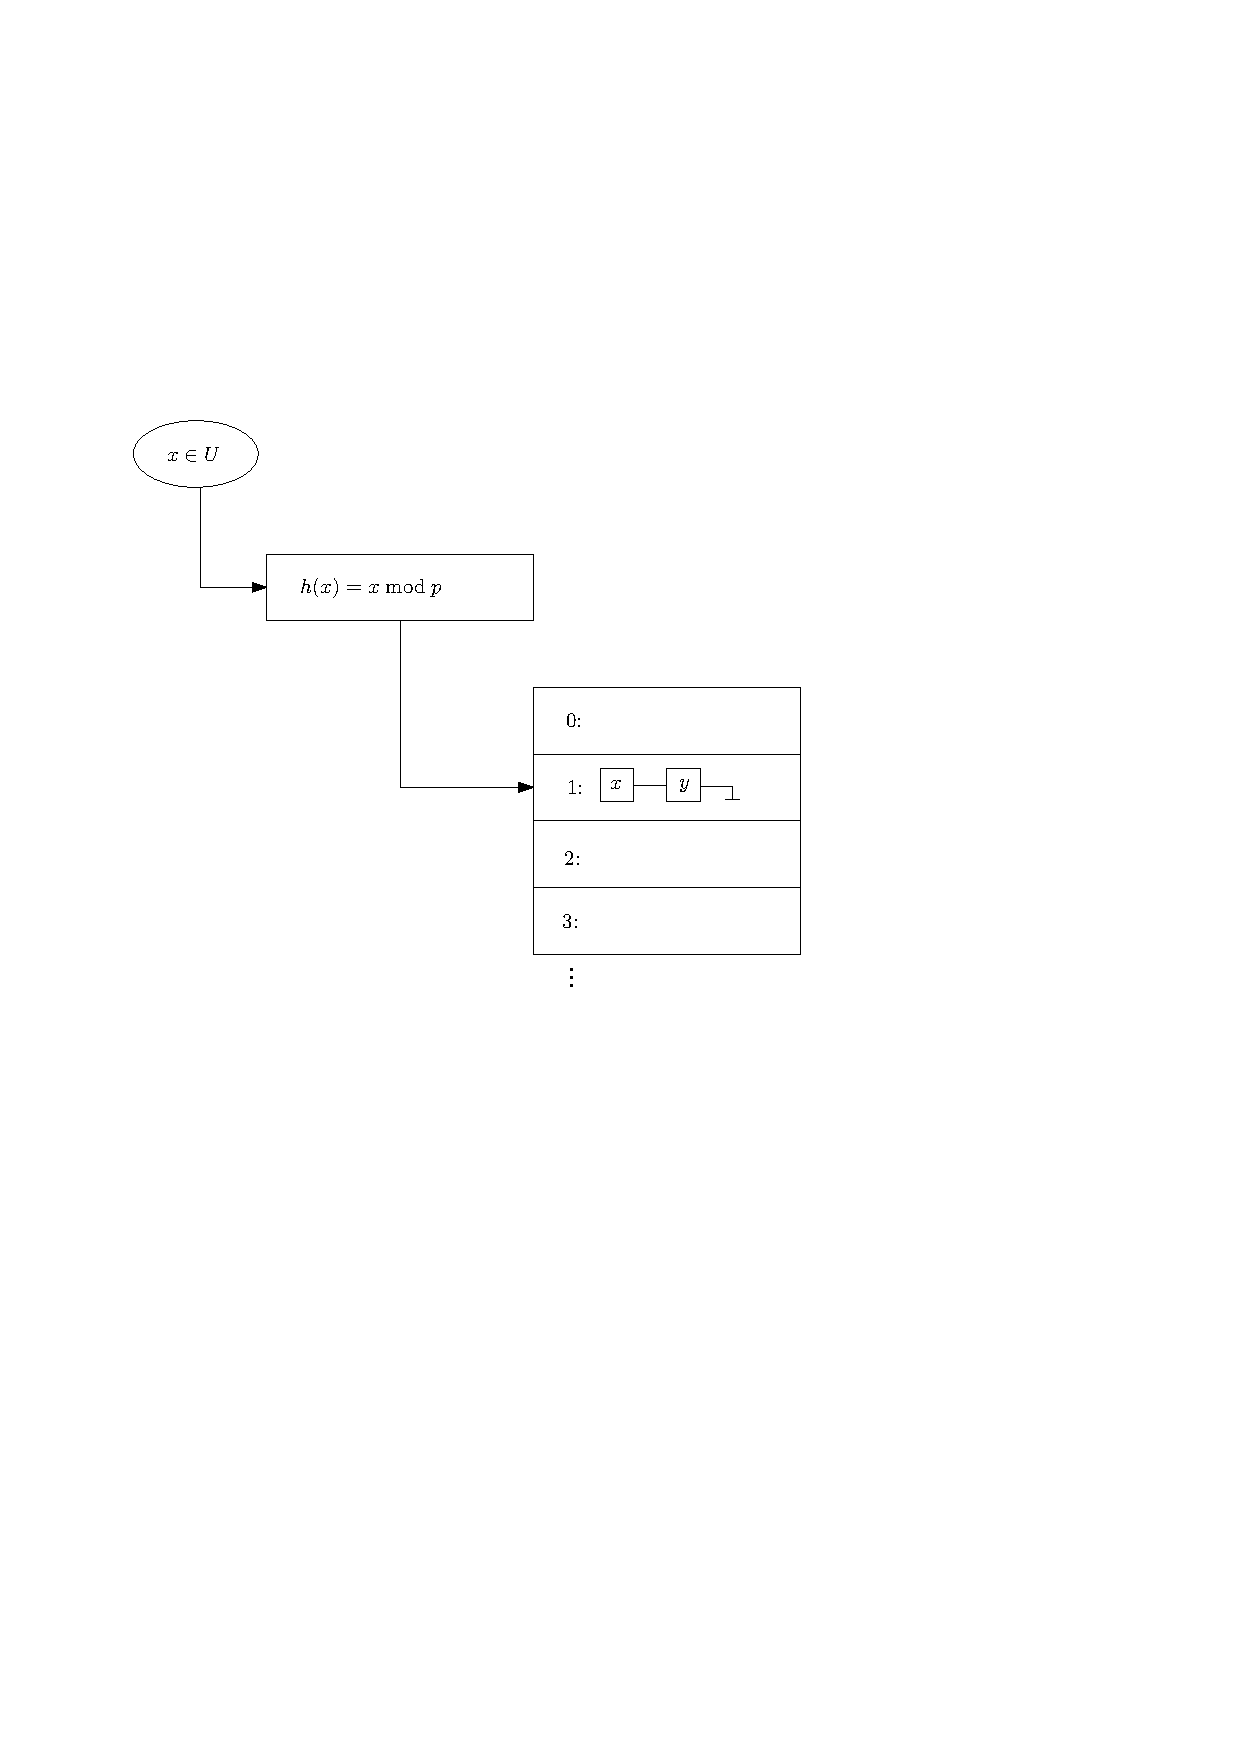
\includegraphics[width=0.5\textwidth]{images/hash_table}
  \caption{Concept of a hash table.}
\end{figure}

If buckets are represented by linked lists, then the expected time of the find operation is proportional to one half of the length of the list.
\begin{lemma}
\label{lemma-expected-list-time}
Let $S$ be a set represented by a linked list. Assume that for every element $x \in S$: \[ \Prob{x \text{ is argument of the find operation}} = \frac{1}{|S|} \text{.} \] Then the expected time of the find operation is $\frac{|S| + 1}{2}$.
\end{lemma}
\begin{proof}
Let $x_i \in S$ be the $i$-th element of the list, $1 \leq i \leq |S|$. Time to find the element $x_i$ inside the list equals $i$. The expected time of the find operation can be expressed directly from its definition. 
\[
\begin{split}
\Expect{\text{time of the find operation}} 
	& = \displaystyle\sum_{i = 1}^{|S|} i \Prob{x_i \text{ is the argument of the find operation}} \\
	& = \frac{\sum_{i = 1}^{|S|}{i}}{|S|} = \frac{|S|(|S| + 1)}{2 |S|} = \frac{|S| + 1}{2} \\
\end{split}
\]
\end{proof}

As seen in the previous lemma the time complexity of an operation needs not to be measured by its worst case time. Compare $|S|$, which is the worst case, to the expected value $\frac{|S| + 1}{2}$ which is better. Considering only the worst case times does not tell much about the structure's real behaviour. We should use probability based characteristics that give more accurate results. These characteristics include the expected operation's time or its expected worst case time which is usually far more difficult to analyse. For hashing this difference means an asymptotic improvement.

\section{Formalisms and Notation}
\label{section-notation}
Notation and formalisms that mathematically describe a hash table are crucial part of an exact analysis. Assume that we are hashing a \emph{universe} $U$ on a \emph{hash table} of size $m$. The table consists of buckets each having its unique address. The addresses are usually quite simple. When the table consists of $m$ buckets the addresses are just $0, \dots, m - 1$. Buckets are always identified by their addresses and thus we can refer to the set $B = \{0, \dots, m - 1\}$ as a hash table.

Universe consists of all the representable elements, examples include the objects of a programming language, strings over an alphabet, numbers or anything else. Hash function is a way to transform these elements into an address of the table, usually a natural number. Hash function $h$ can be described by a function $h: U \rightarrow B$. The other requirements placed on the function $h$ are discussed later.

The letter $S$ typically denotes the \emph{stored set}. We often refer to the variable $n$ as to the size of the stored set, $n = |S|$. As already mentioned we always assume that $S \subset U$ and $|S| \ll |U|$.

Since the universes are really large, recall the previous examples, sizes of the tables are much smaller when compared to those of the universes. Space waste is typically caused by allocating a large table containing many empty buckets. The definition of the table's \emph{load factor} allows an exact analysis of the phenomena connected with the table's filling -- its performance or waste of space.

\begin{definition}[Load factor]
\label{definition-load-factor}
Let $n$ be the size of the represented set and $m$ be the size of the hash table. The variable $\alpha$ defined as \[ \alpha = \frac{n}{m} \] is called the load factor of the table.
\end{definition}

To take control of the table's overhead it is sufficient to keep the load factor in a predefined interval. Not only the empty buckets cause troubles. The overfilled ones are another extreme especially if there are too many collisions.
\begin{definition}[Collision]
\label{definition-collision}
Let $x, y \in U$ be two distinct elements. We say that the elements $x$ and $y$ collide if $h(x) = h(y)$.
\end{definition}

Above all the collision handling is what differentiates distinct hash tables and determines their performance.

To completely explain the notation we have to mention that we refer to the function $\log$ as to the base two logarithm. The function $\ln$ denotes the natural logarithm.

\section{Assumptions of Classic Hashing}
In Lemma \ref{lemma-expected-list-time} we computed the expected time of the find operation and used it as a measure of its time complexity. Known probability distribution of the input enables us to compute the expected value. For the lemma we assumed the uniform distribution. In hashing similar situation occurs. If we want to find the expected results, then we need corresponding probabilistic assumptions on the input. The assumptions we make may be found in \cite{VK-skripta} or in \cite{DBLP:books/sp/Mehlhorn84}. They are similar to ours.
\begin{itemize}
\item Hash function $h$ distributes the elements of universe uniformly across the hash table:
\[
||h^{-1}(x)| - |h^{-1}(y)|| \leq 1 \text{ for every }x, y \in U \text{.}
\]
\item Every set has the same probability of being stored among the sets of the same size:
\[
\Prob{S \text{ is stored}} = \frac{1}{\dbinom{|U|}{|S|}} \text{ for every set } S \subset U \text{.}
\]
\item Every element of the universe has the same probability of being an argument of an operation:
\[
\Prob{x \text{ is used as an argument of an operation}} = \frac{1}{|U|} \text{ for every } x \in U \text{.}
\]
\end{itemize}

These assumptions provides us with a probabilistic model for the average case analysis of classic hashing.

\section{Separate Chaining}
Separate chaining \cite{The-art-of-computer-programming}, \cite{DBLP:books/sp/Mehlhorn84} and \cite{DBLP:books/sp/MehlhornS2008} may be considered the most basic hash table implementation. However, it provides a sufficient framework for illustration of various problems and analyses. Separate chaining usually utilises one hash function mapping elements to an address -- an index of the array representing the hash table. Every represented element is stored within a bucket given by its hash address. Every bucket is represented by a singly linked list. 

Separate chaining, like the other classic models of hashing, is quite dependent on the stored input. The previous assumptions are required for its average case analysis. This model assumes hashing of the universe $U = \{0, \dots, N - 1\}$ for $N \in \mathbb{N}$ into a table of size $m$. Number $m$ is much smaller then $N$ and moreover it is chosen to be a prime. Primality of $m$ improves the ability of the hash function to uniformly distribute the stored set across the table.  Following example clarifies why primality is important for the choice of $m$.

\begin{example}
Consider set $S = \{5n \setdelim n \in \{0, \dots, 5\} \}$ and a table consisting of $10$ buckets. Set $S$ contains only 6 elements, so the table's load factor equals $0.6$. If we use function $x \bmod 10$, then it maps the elements of the set $S$ just onto two addresses, $0$ and $5$. The hash table is not used effectively. Choosing $m$ to be a prime number improves the results but is not a remedy.
\end{example}

The apparent disadvantage of classic hashing is usage of a single hash function known in advance. For example if  the stored set $S$ is chosen, by an adversary, so that $S \subseteq f^{-1}(b)$ for a single bucket $b \in B$, we run into problems. Because our assumptions say that the probability of having such an input is quite low, these inputs may be neglected.

To illustrate how separated chaining works the algorithms are presented. Although the model is quite simple the subroutines regarding the singly linked lists are not discussed. They are considered elementary enough. Remark that their running times are proportional to the length of the represented chain. Notice that the insert procedure has to check if the element is already stored inside the list so that it is not stored twice. 

\begin{algorithm}[ht]
\caption{Find operation of the separate chaining.}
\label{algorithm-find-separate-chaining}
\floatname{algorithm}{Procedure}
\begin{algorithmic}
\REQUIRE $x \in U$
\STATE $h = h(x)$
\STATE
\IF {$T\left[h\right] \text{ contains } x$}
	\RETURN \textbf{true} \COMMENT{operation is successful}
\ELSE
	\RETURN \textbf{false} \COMMENT{operation is unsuccessful}
\ENDIF
\end{algorithmic}
\end{algorithm}

\begin{algorithm}[ht]
\caption{Insert operation of the separate chaining.}
\label{algorithm-insert-separate-chaining}
\floatname{algorithm}{Procedure}
\begin{algorithmic}
\REQUIRE $x \in U$
\STATE $h = h(x)$
\STATE
\IF {$T\left[h\right] \text{ does not contain } x$}
	\STATE insert $x$ into chain $T[h]$
\ENDIF
\end{algorithmic}
\end{algorithm}

\begin{algorithm}[ht]
\caption{Delete operation of the separate chaining.}
\label{algorithm-delete-separate-chaining}
\floatname{algorithm}{Procedure}
\begin{algorithmic}
\REQUIRE $x \in U$
\STATE $h = h(x)$
\STATE
\IF {$T\left[h\right] \text{ contains } x$}
	\STATE remove $x$ from chain $T[h]$
\ENDIF
\end{algorithmic}
\end{algorithm}

\begin{theorem}[Average case of the separate chaining]
Let $\alpha > 0$ be the load factor of the hash table resolving collisions by separate chaining. Then the expected time of the successful find operation converges to $1 + \frac{\alpha}{2}$ and to $e^{-\alpha} + \alpha$ in the unsuccessful case.
\end{theorem}
\begin{proof}
The theorem is proved in \cite{DBLP:books/sp/Mehlhorn84}.
\end{proof}

Various modifications of separate chaining are known. If the universe is an ordered set then ordering the elements in chains monotonously may bring a speedup. This is caused by the fact that the operations concerning the chains do not have to iterate throughout the whole list and stop earlier. 

There is a modification utilising the move to front principle \cite{723912}. This principle is motivated by the rule of the locality of reference \cite{DBLP:books/aw/AhoSU86}. The rule says that whenever an element is accessed, it is very likely that it is going to be accessed again in a short future. Therefore it is quite convenient to put the last accessed element to the front of the list so that it is accessed fast.

Another set of modifications changes the representation of chains. They are no longer represented by common linked lists since their cache behaviour \cite{1200662} is poor as stated in \cite{Rubin99virtualcache}. The chains are stored directly in the hash table. So when resolving a collision an empty place in the hash table is taken. There are problems connected with this approach that need to be solved. Above all chains may not be merged together. This appears when a new chain should be started but the place of the first element is already taken. It may be solved by moving the element, not belonging to the chain, to another empty place. To perform the replacement quickly we are forced to use double linkage. Or, instead of using doubly linked lists, at every address an additional begin pointer may point to the first element of the chain. In addition, we have to deal with the fact that schemes using only the hash table suffer from bad behaviour when the load factor is almost one. And of course a uniform random choice of an empty bucket has to be provided when prolonging a chain.

\section{Coalesced Hashing}
In coalesced hashing, the chains of colliding elements are also stored directly in the hash table. However, they are allowed to fuse together. Every chain is represented by a singly linked list. The simpler methods such as LISCH and EISCH do not use any special additional memory. In addition, the EISCH method utilises the move to front rule. Methods such as LICH, EICH and VICH use the additional memory which is not directly addressable by the hash function. Collision resolution uses the additional memory to store growing chains. When an empty place for a colliding element is needed, it is first sought in the additional memory. Only if the special memory is full, then the addressable memory is used. The methods are distinct in a way they use the move to front rule. The EICH method always obeys it, VICH uses it only in the addressable memory and the LICH method does not obey the rule at all.

\begin{figure}
  \centering
    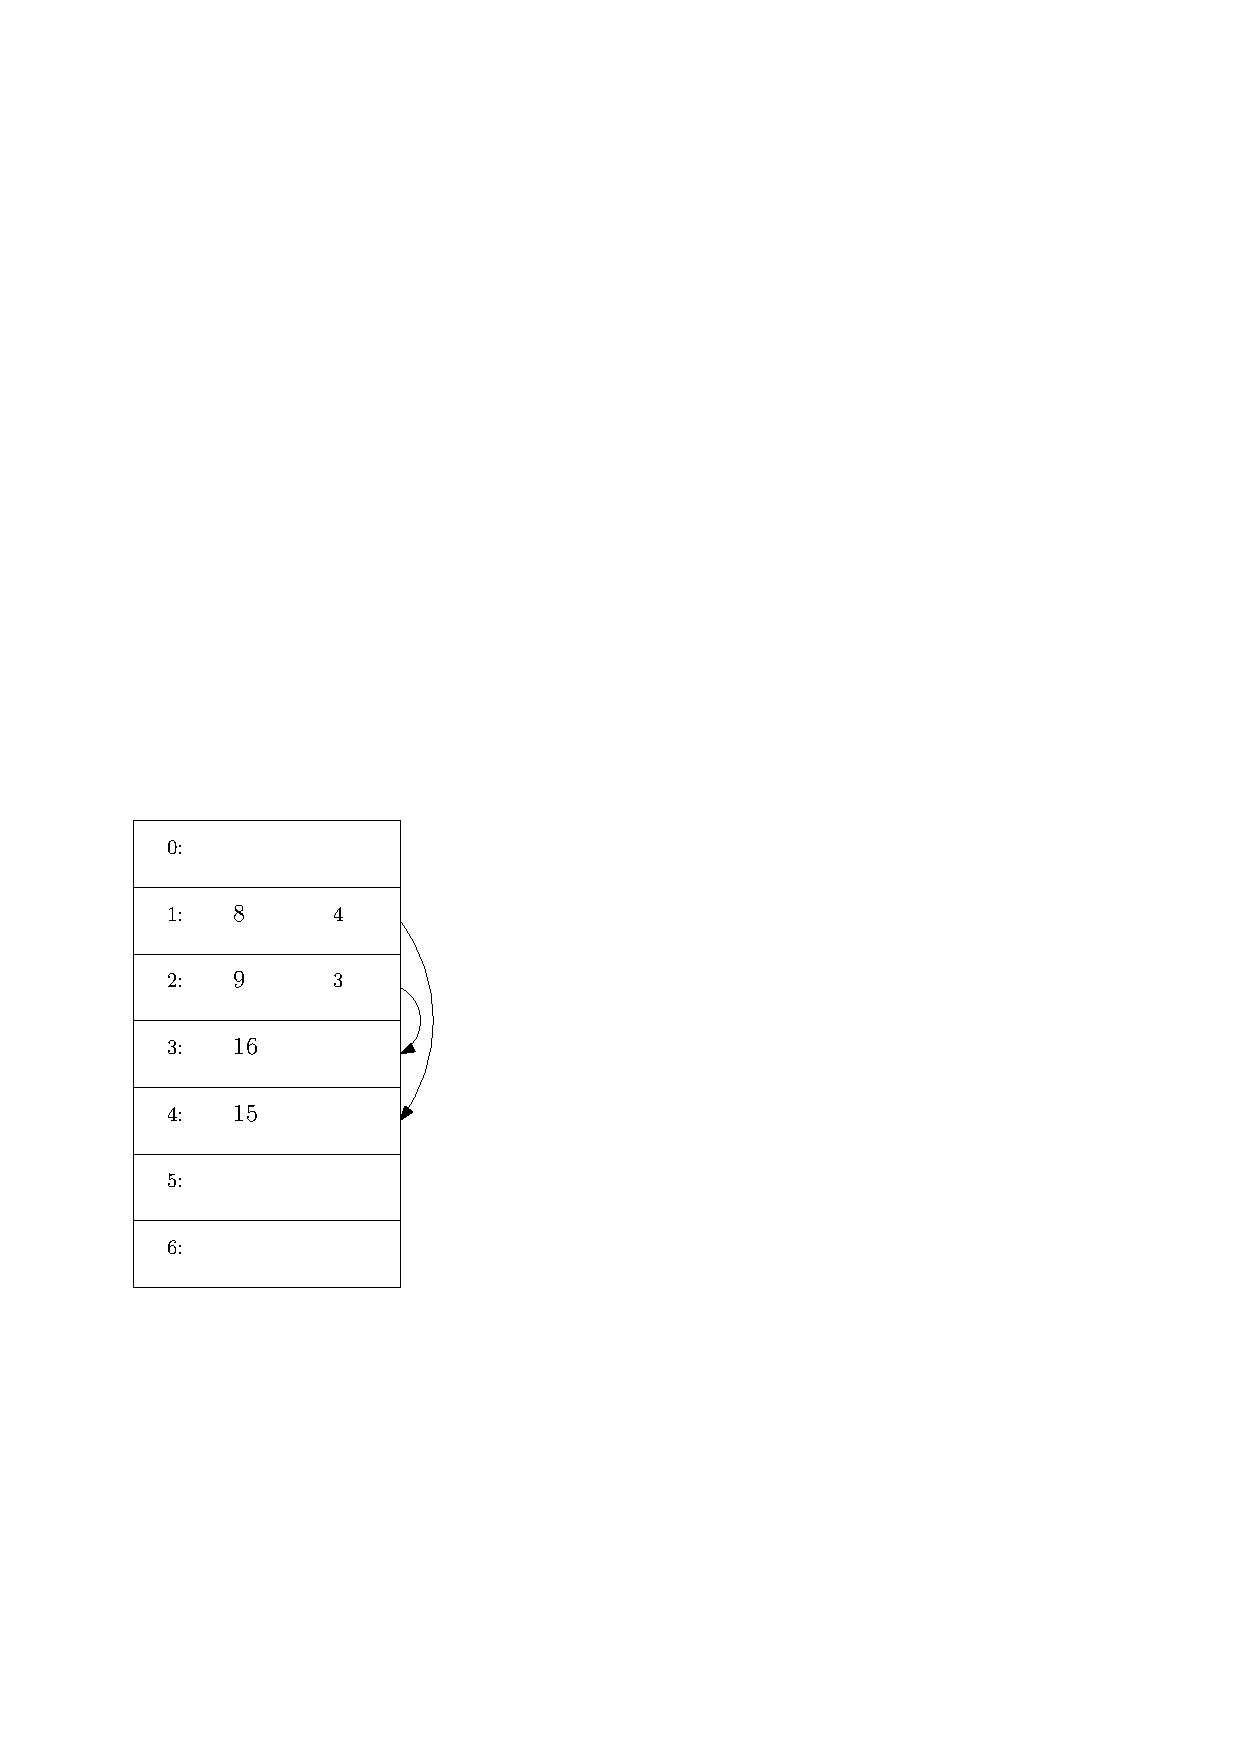
\includegraphics[width=0.2\textwidth]{images/vich}
  \caption{Singly linked lists represented directly in the hash table. The first number is the bucket's address, the second is the represented key and the last one is the next pointer.}
\end{figure}

\section{Open Addressing}
Methods of coalesced hashing and separate chaining represent the chains explicitly by linked lists. The additional pointer of the list not only consumes an extra memory. It also worsens the cache behaviour of the hash table. Open addressing also merges the chains together. They are stored directly in the hash table and their representation is more implicit. To remove the need of an additional pointer, a secondary function for conflict resolution is used.

Models of open addressing assume existence of two hash functions $h_1: U \rightarrow B$ and $h_2: U \rightarrow B$. Assume $x \in U$ is the $i$\textsuperscript{th} element of the chain and the order of elements in a chain starts from zero. Its address is then determined by a compound hash function $h(x, i) = h_1(x) + i h_2(x)$. When we insert the element $x \in U$ we find a minimal $i$ such that the bucket at the address $h(x, i)$ is empty.

This approach also removes the problem of the choice of a free bucket when a collision occurs. Unfortunately, there is no fast implementation of the delete operation known so far. To delete an element we can mark its bucket as free and reuse it when possible. Marking the deleted element's bucket is necessary if we do not want to accidentally loose the elements lying behind the deleted one in the chain.

\subsection{Linear Probing}
Linear probing is a scheme of open addressing with $h_2(x) = 1$ for every $x \in U$. The last element of the prolonged chain is placed into the first empty bucket behind the one with the address $h_1(x)$.

Another problem of linear hashing is its degradation. Clusters of non-empty buckets emerge when load factors reach one. Delete operation implemented by marking only emphasises this problem.

\subsection{Double Hashing}
If we want to distribute the stored set uniformly across the hash table, then the choice of a free bucket should be random. Whenever function $h(x, i)$ of argument $i$ is a random permutation of $B$, then the mentioned choice becomes random. A necessary condition is that $h_2(x)$ and $m$ are incommensurable. Therefore the size of the hash table is chosen so that it is a prime number again. 

Double hashing has theoretical analyses yielding remarkable results.
\begin{theorem}
Let $\alpha \in (0, 1)$ be the load factor of the hash table resolving collisions by double hashing. Then the running time of the find operation  converges to $\frac{1}{1 - \alpha}$ in the unsuccessful case and to $\frac{1}{\alpha}\log\left(\frac{1}{1 - \alpha}\right)$ when the operation is successful.
\end{theorem}
\begin{proof}
The proof is shown in \cite{DBLP:books/sp/Mehlhorn84}.
\end{proof}

\section{Universal Hashing}
Universal hashing uses a universal system of functions instead of a single function. This removes the dependence of universal hashing on its input. The probability space is now determined by the uniform choice of the hash function instead of selection of a stored set. We study universal hashing and its systems in Chapter \ref{chapter-universal-classes} in a more detail way.

\section{Perfect Hashing}
Assume that the stored set $S$ is known in advance. The problem solved by perfect hashing is how to create a hash table and a hash function such that the find operation takes only a constant time. Insert and delete operations are forbidden, the stored set $S$ remains fixed. Additional requirements are placed on the size of the scheme. Size of the hash table is not the only problem. We must also take care about the space needed to represent the constructed hash function since it becomes quite complex.

\section{Modern Approaches}
Modern approaches to hashing are nowadays often based on their probabilistic properties. Authors adapt and change their models to improve the asymptotic results in the average case and in the expected worst case. The algorithms still remain fast and are enriched by simple rules. 

Straightforward use of a single function is not enough and various universal systems are used. Theoretical analyses of the models do not necessarily involve the ideas of universal hashing. Universal classes are used as an heuristic. Although the algorithms are not complicated, their analyses become more and more difficult.

A model called \emph{robin hood hashing} \cite{10.1109/SFCS.1985.48}, \cite{Devroye04onworst} is an improvement of the double hashing. In double hashing we are able to access the chain at an arbitrary position in constant time. The main idea of robin hood hashing is to minimise the variance of the expected chain length. If probing starts from the average chain length the expected time of the find operation becomes constant.

Another model, \emph{hopscotch hashing} \cite{DBLP:conf/wdag/HerlihyST08}, is a modification of the linear probing utilising the computer's cache behaviour. A chain is kept together in one place as long as possible. Algorithms in control of the processor cache store whole blocks of memory inside it when only a single part of the block is accessed. Provided that the chains are compact, storing them in the cache is quite probable. This optimisation makes probing substantially faster.

Next investigated model is \emph{cuckoo hashing} \cite{782440}. However, the interest fades these days since there are some problems connected with it \cite{DBLP:conf/sofsem/DietzfelbingerS09}, \cite{1496857}.

\chapter{Systémy univerzálnych funkcií}

% TODO: Odkazy na jednotlive systemy
% TODO: Citacia na clanok s definiciami.

\begin{definition}[Silne $n$-univerzálny systém hashovacích funkcií]
\label{strong_universal_n_system}
Nech $n \in N$ a $H$ je množina funkcií $h: U \rightarrow A$ taká, že pre každé $x_1, x_2, \dots, x_n \in U$, $x_i \neq x_j$ pre $i \neq j$ a $y_1, y_2, \dots, y_n \in A$ platí $\left|\lbrace h \in H | h(x_1) = y_1, h(x_2) = y_2, \dots, h(x_n) = y_n \rbrace \right| = \frac{|H|}{|A|^n}$. Potom systém funkcií $H$ nazveme silne $n$-univerzálny.
\end{definition}

\begin{definition}[Silne $2$-univerzálny systém hashovacích funkcií]
\label{strong_universal_2_system}
Systém funkcií $H$ je silne $2$-univerzálny, pokiaľ je silne univerzálny pre $n = 2$.
\end{definition}

\begin{definition}[Silne $\omega$-univerzálny systém hashovacích funkcií]
\label{strong_universal_omega_system}
Systém funkcií $H$ je silne $\omega$-univerzálny, pokiaľ je silne univerzálny pre každé $n \in N$.
\end{definition}

% TODO: Citacia na clanok o systeme omega univerzalnych funkcii.
Toto je veľmi silná požiadavka kladená na systém funkcií. Jednoduchým prí\-kladom je množina všetkých funkcií z univerza $U$ do $A$. Ide o prakticky neveľmi použiteľný systém kvôli veľkosti potrebnej na jeho kódovanie. 

\begin{definition}[$c$-univerzálny systém hashovacích funkcií]
\label{c_universal_system}
Nech $c \in R, c > 0$, a $H$ je množina zobrazení $h: U \rightarrow A$ taká, že každú dvojicu $x, y \in U$, $x \neq y$ je $\left| \lbrace h \in H | h(x) = h(y) \rbrace \right| \leq \frac {c |H|}{|A|}$. Potom $H$ nazveme $c$-univerzálny systém hashovacích funkcií.
\end{definition}

\begin{remark}
Každý silne $2$-univerzálny systém funkcií je $1$-univerzálny.
\end{remark}
\begin{proof}
Nech $x, y \in U$ sú dané. Aby platilo $h(x) = h(y)$ postupne volíme všetky $t \in A$ tak, že $h(x) = h(y) = t$. Množiny funkcií $H_t = \lbrace h \in H | h(x) = h(y) = t \rbrace$ sú navzájom disjunktné a navyše $|H_t| = \frac{|H|}{{|A|}^{2}}$. Zvolili sme oba obrazy rovné $t$. Po sčítaní cez všetky $t \in A$ dostávame:
\begin{displaymath}
|\lbrace h \in H | h(x) = h(y) \rbrace | = \displaystyle \sum_{t \in A} |H_t| = |A| \frac{|H|}{{|A|}^{2}} = \frac{H}{|A|}
\end{displaymath}
\end{proof}

\begin{remark}
Každý silne $n$-univerzálny systém funkcií je silne $k$-univerzálny pre každé $1 \leq k \leq n$.
\end{remark}
\begin{proof}
Použijeme rovnaký prístup ako v predchádzajúcom prípade. Nech máme zadaných $k$ po dvojiciach rôznych vzorov $x_1, \dots, x_k \in U$ a k nim odpovedajúce obrazy $y_1, \dots, y_k$. 
\begin{itemize}
\item Postupnosť vzorov rozšírime pomocou ďalších ľubovoľných $n - k$ ale rôznych prvkov na $n$ prvkovú. 
\item K množine obrazov budeme voliť všetky možné $(n-k)$-tice prvkov z $A$. 
\end{itemize}
Pretože nám nezáleží na obrazoch vzorov, ktoré sme pridali, platí:
\begin{displaymath}
\lbrace h \in H | h(x_i) = y_i, i \in \lbrace 1, \dots, k \rbrace \rbrace = \displaystyle \bigcup_{y_{k+1}, \dots, y_n \in A} \lbrace h \in H | h(x_i) = y_i, i \in \lbrace 1, \dots, n \rbrace \rbrace
\end{displaymath}
Množiny funkcií, ktoré zobrazujú množinu rozšírených vzorov na zvolené obrazy, sú navzájom disjunktné:
\begin{displaymath}
\begin{split}
\left| \lbrace h \in H | h(x_i) = y_i, i \in \lbrace 1, \dots, k \rbrace \rbrace \right| 
	& = \left| \displaystyle \bigcup_{y_{k+1}, \dots, y_n \in A} \lbrace h \in H | h(x_i) = y_i, i \in \lbrace 1, \dots, n \rbrace \rbrace \right|  \\
	& = \displaystyle \sum_{y_{k+1}, \dots, y_n \in A} \left| \lbrace h \in H | h(x_i) = y_i, i \in \lbrace 1, \dots, n \rbrace \rbrace \right| \\
	& = \displaystyle \sum_{y_{k+1}, \dots, y_n \in A} \frac{H}{{|A|}^{n}} = {|A|}^{n - k} \frac{H}{{|A|}^{n}} = \frac{H}{{|A|}^{k}}
\end{split}
\end{displaymath}
\end{proof}

% Linear systems
\paragraph{Lineárny systém}
\begin{definition}[Lineárny systém]
Nech $U = \{0, \dots, N - 1 \}$ a $A = \{0, \dots, m - 1\}$. Potom systém funkcií 
\[ H = \{h(x): U \rightarrow A | h(x) = ((ax + b) \mod N) \mod m\} \]
nazveme lineárny systém hashovacích funkcií.
\end{definition}

\begin{remark}
Lineárny systém je $\frac{\left(\left\lceil \frac{N}{m} \right\rceil\right)^2}{\left(\frac{N}{m}\right)^2}$-univerzálny.
\end{remark}
% End linear systems

% Linear transformations
\paragraph{Systém lineárnych zobrazení}
\begin{definition}{Systém lineárnych zobrazení}
Nech $A$, $B$ sú dva vektorové priestory nad $Z_2$ pričom platí $dim(A) = m$ a $dim(B) = n$. Systém funkcií 
\begin{displaymath}
H = \{L : A \rightarrow B | L \text{ je lineárne zobrazenie}\}
\end{displaymath}
nazveme systém lineárnych zobrazení.
\end{definition}
\begin{remark}
Systém lineárnych zobrazení je $1$-univerzálny.
\end{remark}
\begin{proof}
Označme $(T)_{i, j}=t_{i, j}$ ako maticu lineárneho zobrazenia. Máme zadané dva rôzne prvky $x$, $y$ z priestoru $A$, nech sa líšia na $k$-tom mieste. Nech všetky prvky matice $T$ okrem $k$-teho stĺpca sú definované. Teraz sme schopní jednoznačne určiť ostávajúce hodnoty, pre, $1 \leq i \leq n$, $i$-ty riadok máme:
\begin{displaymath}
\begin{split}
\displaystyle\sum_{j = 1}^{m}t_{i, j}x_j & = \displaystyle\sum_{j = 1}^{m}t_{i, j}y_j \\
t_{i, k} & = (x_k - y_j)^{-1}\displaystyle\sum_{j = 1, j \neq k}^{m}t_{i, j}(y_j - x_j)
\end{split}
\end{displaymath}
Teda $k$-ty stĺpec môžeme jednoznačne určiť. Počet všetkých funkcií je $2^{mn}$ a kolíznych zobrazení je $2^{(m-1)n}$.
\begin{displaymath}
2^{(m-1)n} = \frac{2^{mn}}{2^n}
\end{displaymath}
Systém lineárnych zobrazení je $1$-univerzálny.
\end{proof}
% End linear transformations

% Polynoms
\paragraph{Polynómy nad konečnými poliami}
\begin{definition}[Polynómy nad konečnými poliami]
Nech $U = \{0, \dots, N - 1 \}$, $A = \{0, \dots, m - 1\}$ a $n \in N$. Potom systém funkcií 
\[ H = \{h(x): U \rightarrow A | h(x) = ((\displaystyle \sum_{i=0}^{n} c_i x^i ) \mod N) \mod m\} \]
nazveme systém polynomiálnych hashovacích funkcií stupňa $n$. Koeficienty $c_i, i \in \{0, 1, \dots, n\}$ volíme z množiny $U$.
\end{definition}
\begin{remark}
Nech $N$ je prvočíslo. Systém polynomiálnych hashovacích funkcií stupňa $n$ je silne $n + 1$-univerzálny pre $A = U$. Pre $A \neq U$ je "takmer" silne $n + 1$-univerzálny.
\end{remark}
\begin{proof}
% TODO: Odkaz na Vandermondovu maticu.
Nech prvky $x_1, x_2, \dots, x_{n+1}$ sú po dvojiciach rôzne a $y_1, y_2, \dots, y_{n+1}$ sú zvolené odpovedajúce obrazy. Potom môžeme zostaviť Vandermondovu maticu pre určenie jednotlivých koeficientov $c_0, c_1, \dots, c_n$.

Pokiaľ $U = A$, funkcie $h(x)$ sa redukujú na tvar $h(x) = (\displaystyle \sum_{i=0}^{n} c_i x^i ) \mod N$. Veľkosť systému je ${|U|}^{n+1}$. Pre zadané vzory a ich obrazy z invertibility Vanderomondovej matice dostávame práve jednu funkciu $h$, ktorá spĺňa predpísané podmienky. Za predpokladu $|A| = |U|$ platí ${|A|}^{n+1} = {|U|}^{n+1}$. Ihneď získavame, že systém polynomiálnych funkcií je silne $n+1$-univerzálny.

Teraz nech $U \neq A$. Postupujeme obdobne ako v dôkaze $c$-univerzality lineárneho systému.
\begin{displaymath}
(\displaystyle \sum_{j=0}^{n} c_j x_{i}^{j} ) \mod N = {y}_i + {r_i}{m} \qquad {y}_i \in \{0, \dots, m - 1 \}, r_i \in \{0, m, 2m, \dots, \left\lceil \frac{N}{m} \right\rceil - 1\}
\end{displaymath}
Pre každú voľbu ${y}_i$ a $r_i$ dostávame jednoznačné riešenie sústavy. Pokiaľ sú zadané obrazy $y_i$, hodnoty $r_i$ už môžu byť ľubovoľné. Pre každú voľbu $r_i$ máme jedinú funkciu spĺňajúcu zadané predpoklady. Počet sád $r_i$ je ${\left\lceil \frac{N}{m} \right\rceil}^{n + 1}$ a práve toľko je polynomiálnych hashovacích funkcií, ktoré pošlú zadané vzory na im príslušné obrazy.
\begin{displaymath}
|\{h \in H | h(x_i) = y_i, i \in \{1, \dots, n + 1\}\}| = {\left\lceil \frac{N}{m} \right\rceil}^{n + 1} = \frac{{\left\lceil \frac{N}{m} \right\rceil}^{n + 1}}{(\frac{N}{m})^{n+1}}\left(\frac{N}{m}\right)^{n+1}
\end{displaymath}
\end{proof}
% End polynoms


\paragraph{Bitový súčet reťazca nad konečným poľom}
\begin{definition}
Nech $U = \{0, \dots, N - 1\}$ a $A = \{0, \dots, p - 1 \}$, kde $N = 2^k$ a $p$ je prvočíslo, zvolíme $l \leq p$. Pre každý prvok $x \in U$ budeme chápať zápis $x = x_{k - 1} x_{k-2} \dots x_0$ ako zápis čísla x v binárnej sústave ($x = \displaystyle \sum_{j=0}^{k-1} x_j 2^j$). Systém funkcií 
\begin{displaymath}
H = \{ h: U \rightarrow A | h(x) = (\displaystyle \sum_{i=0}^{k-1} c_i x_i) \mod p, c_i \in \{0, 1, \dots, l - 1\} \}
\end{displaymath} 
nazveme reťazcový systém.
\end{definition}
\begin{remark}
Reťazcový systém je $c$-univerzálny, pre $c = \frac{p}{l}$.
\end{remark}
\begin{proof}
Vieme, že $|H| = l^k$. Nech $x, y \in U$ a $x \neq y$, existuje $0 \leq j \leq k-1$, t.ž. $x_j - y_j \neq 0$.
Nech $h(x) = h(y)$, potom:
\begin{displaymath}
\begin{split}
\left(\displaystyle \sum_{i=0}^{k-1} c_i x_i\right) \mod p & = \left(\displaystyle \sum_{i=0}^{k-1} c_i y_i\right) \mod p \\
c_j(x_j - y_j) \mod p & = \left(\displaystyle \sum_{i=0, i \neq j}^{k-1} c_i (x_i - y_i)\right) \mod p \\
c_j & = (x_j - y_j) ^ {-1}\left(\displaystyle \sum_{i=0, i \neq j}^{k-1} c_i (x_i - y_i)\right) \mod p
\end{split}
\end{displaymath}
Posledná rovnosť platí, pretože $p$ je prvočíslo a prvok $x_j - y_j$ je invertibilný. Pri výbere funkcií, ktoré dané dva rôzne prvky nechajú kolidovať, sme o voľbu jednej konštanty $c_j$ ochudobnení. 

\begin{displaymath}
|\{h \in H | h(x) = h(y) \}| = l^{k-1} = \frac{p}{l}\frac{l^k}{p} = c\frac{|H|}{|A|}
\end{displaymath}
\end{proof}

% All functions
\paragraph{Množina všetkých zobrazení}
\begin{remark}
Systém všetkých zobrazení $h: U \rightarrow A$ je silne $\omega$-univerzálny.
\end{remark}
\begin{proof}
Platí:
\begin{displaymath}
|H| = {|A|}^{|U|}
\end{displaymath}
Nech máme zadaných $n$ po dvojiciach rôznych vzorov $x_1, \dots, x_n$ a im odpovedajúce obrazy $y_1, \dots, y_n$. Veľkosť $H_n = \lbrace h \in H | h(x_i) = y_i, i \in \lbrace 1, \dots, n \rbrace \rbrace$ je:
\begin{displaymath}
|H_n| = {|A|}^{|U| - n} = \frac{{|A|}^{|U|}}{{|A|}^{n}} = \frac{|H|}{|A|^n}
\end{displaymath}
\end{proof}

Pamätať si úplné zobrazenie zo systému $H$ je nepraktické. Kódujeme aj hodnoty prvkov, ktoré sa nikdy v hashovanej množine nevyskytnú. Alternatívou je konštruovať náhodnú parciálnu funkciu z množiny všetkých zobrazení z $U$ do $A$ nasledujúcim spôsobom. Vychádzame z predpokladu existencie rýchlej asociatívnej pamäti a generátora náhodných prvkov. Kedykoľvek máme hashovať prvok, tak chceme určiť hodnotu hashovacej funkcie. Najprv pomocou asociatívnej pamäti zistíme, či už nemá priradenú hodnotu. Ak nie, vygenerujeme náhodný prvok z množiny $A$ a do asociatívnej pamäti toto zobrazenie poznamenáme. Jedná sa o postupnú konštrukciu funkcie z množiny všetkých zobrazení. Nakoľko táto konštrukcia vyberá prvky rovnomerne, zostrojená funkcia má vlastnosti silne $\omega$-univerzálneho systému. Navyše nemáme uložené mapovanie pre prvky, ktoré sme doteraz nepotrebovali.
% End all functions

\paragraph{Malý univerzálny systém}


\paragraph{Systém definovaný pomocou matíc}

\chapter{Očakávaná dĺžka najdlhšieho reťazca}

Pokúsime sa odhadnúť očakávanú dĺžku najdlhšieho reťazca, značíme ako náhodnú veličinu $lpsl$,  pri univerzálnom hashovaní. Vychádzame z postupu použitého pri štandardnom hashovaní, ktorý neskôr upravíme. Pri tomto prístupe sme očakávanú dĺžku odhadovali pomocou pravdepodobnosti, že v jedinom reťazci koliduje $i$ a viac prvkov. Vychádzali sme z nasledujúcich dvoch faktov:
\begin{displaymath}
P(lpsl \geq i) \leq m P(psl \geq i)
\end{displaymath}

\begin{displaymath}
\begin{split}
E lpsl	& = \displaystyle \sum_{i=0}^{\infty} i P(lpsl = i) \\
		& = \displaystyle \sum_{i = 0}^{\infty} i (P(lpsl \geq i) - P(lpsl \geq i + 1)) \\ 
		& = \displaystyle \sum_{i = 0}^{\infty} P(lpsl \geq i)
\end{split}
\end{displaymath}

Teda platí:
\begin{displaymath}
E lpsl \leq \displaystyle \sum_{i = 0}^{\infty} m P(psl \geq i)
\end{displaymath}

Z platnosti predpokladu nezávislosti výberu hashovaných prvkov z univerza od\-had\-ne\-me pravdepodobnosť kolízie ako:
\begin{displaymath}
P(psl \geq i) \leq \dbinom{n}{i}\left(\frac{1}{m}\right)^i\left(1 - \frac{1}{m}\right)^{n-i}
\end{displaymath}

Dopočítame odhad očakávanej dĺžky najdlhšieho reťazca:
\begin{displaymath}
\begin{split}
E lpsl	& \leq \displaystyle \sum_{i = 0}^{\infty} m P(psl \geq i) \\
		& \leq \displaystyle \sum_{i = 0}^{\infty} m \dbinom{n}{i}\left(\frac{1}{m}\right)^i\left(1 - \frac{1}{m}\right)^{n-i} \\
		& = O(\frac{\log n}{\log \log n})
\end{split}
\end{displaymath}

Teraz upravíme výpočet pre univerzálne hashovanie. Zásadný rozdiel je v odhade pravdepodobnosti kolízie $i$ prvkov. Tu sa oprieme o rôzne definície univerzálnych systémov hashovacích funkcií a o špecifické vlastnosti jednotlivých sád funkcií.

\begin{definition}[Indikátor]
\begin{displaymath}
I: P(U) \rightarrow \lbrace 0, 1 \rbrace
\end{displaymath}
\begin{displaymath}
I(M) = \left\{ 
\begin{array}{l l}
  0 & \quad M = \emptyset \\
  1 & \quad M \neq \emptyset \\
\end{array} \right.
\end{displaymath}
\end{definition}

Z predchádzajúcej definície je vidieť, že platí $I(M) \leq |M|$.

\paragraph{}
Ďalej sa pokúsime načrtnúť výpočet očakávanej dĺžky najdlhšieho reťazca pre univerzálne hashovanie. Nech $h \in H$, $k \in N_0$ a $\tilde{x} \in A$, potom pre
\begin{displaymath}
\begin{split}
M_{\geq k} & = \{Y \subseteq S | |Y| \geq k, h(Y) = \{\tilde{x}\}\} \\
M_{= k} & = \{Y \subseteq S | |Y| = k, h(Y) = \{\tilde{x}\}\} 
\end{split}
\end{displaymath}
platí:
\begin{displaymath}
I(M_{\geq k}) = I(M_{= k})
\end{displaymath}
Chceme ukázať, že neprázdnosť množiny $M_{\geq k}$ je ekvivalentná s neprázdnosťou $M_{= k}$. Nech $M_{\geq k}$ je neprázdna:
\begin{displaymath}
Y \in M_{\geq k} \Rightarrow \forall Y' \subseteq Y, |Y'| = k: h(Y') = \{\tilde{x}\} \Leftrightarrow \forall Y' \subseteq Y, |Y'| = k: Y' \in M_{=k}
\end{displaymath}
Nech $M_{=k}$ je neprázdna:
\begin{displaymath}
Y' \in M_{=k} \Rightarrow Y' \in M_{\geq k}
\end{displaymath}
Máme:
\begin{displaymath}
\begin{split}
M_{\geq k} \neq \emptyset & \Leftrightarrow  M_{= k} \neq \emptyset \\
I(M_{\geq k}) & = I(M_{= k})
\end{split}
\end{displaymath}

Zvolíme reťazec obsahujúci prvok $\tilde{x}$ a jeho dĺžku označíme $l_{\tilde{x}}$. Ak má príslušný reťazec dĺžku aspoň $k$, potom musí existovať podmnožina $Y$ hashovanej množiny $S \subset U$ taká, že použitá funkcia $h$ je na nej konštantne rovná $\tilde{x}$. Aby bola dĺžka zvoleného reťazca presne $k$, množina $Y$ musí byť maximálna čo do počtu prvkov.
\begin{displaymath}
\begin{split}
P(l^{\tilde{x}} \geq k) & = \frac{\sum\displaylimits_{h \in H} I(\{ Y \subseteq S | |Y| \geq k, h(Y) = \{ \tilde{x} \} \})}{|H|} \\
P(l^{\tilde{x}} = k) & = \frac{\sum\displaylimits_{h \in H} I(\{ Y \subseteq S | |Y| = k, h(Y) = \{ \tilde{x} \}, Y \text{ maximálna} \})}{|H|} \\
\end{split}
\end{displaymath}

K tomuto výpočtu je nutné dodať niekoľko užitočných poznámok:
\begin{itemize}
\item Reťazec máme vždy určený jediným prvkom $\tilde{x}$, ktorý do neho patrí.
\item Pravdepodobnosť počítame pre jedinú fixovanú hashovanú množinu $S$ a pravdepodobnostný priestor odpovedá voľbe funkcie $h$.
\item Získame odhad $P(l^{\tilde{x}} \geq k) \leq p(A, U)$. Tento odhad použijeme obdobne ako pri výpočte v klasickom hashovaní na odhad pravdepodobnosti pre dĺžku najdlhšieho reťazca: $P(lpsl \geq k) \leq |A| p(A, U)$.
\end{itemize}
\begin{displaymath}
\begin{split}
P(l^{\tilde{x}} \geq k) 
	& = \frac{\sum\displaylimits_{h \in H} I(\{ Y \subseteq S | |Y| \geq k, h(Y) = \{ \tilde{x} \} \})}{|H|} \\
	& = \frac{\sum\displaylimits_{h \in H} I(\{ Y \subseteq S | |Y| = k, h(Y) = \{ \tilde{x} \} \})}{|H|} \\
	& \leq \frac{\sum\displaylimits_{h \in H} |\{ Y \subseteq S | |Y| = k, h(Y) = \{ \tilde{x} \} \}|}{|H|} \\
	& = \frac{|\{ (h, Y) | |Y| = k, h(Y) = \{ \tilde{x} \} \}|}{|H|} \\
	& = \frac{\sum\displaylimits_{Y \subseteq S, |Y| = k} | \{ h \in H | h(Y) = \{\tilde{x}\} \}|}{|H|} \\
\end{split}
\end{displaymath}
Tento odhad silne závisí na vlastnostiach množiny funkcií $H$.
\begin{theorem}
Pokiaľ $H$ je silne $\omega$-univerzálny systém, očakávaná dĺžka najdlhšieho reťazca pri univerzálnom hashovaní je $O(\frac{\log n}{\log \log n})$.
\end{theorem}
\begin{proof}
\begin{displaymath}
\begin{split}
P(l^{\tilde{x}} \geq k) 
	& \leq \frac{\sum\displaylimits_{Y \subseteq S, |Y| = k} | \{ h \in H | h(Y) = \{\tilde{x}\} \}|}{|H|} \\
	& = \frac{\sum\displaylimits_{Y \subseteq S, |Y| = k} \frac{|H|}{{|A|}^{k}}}{|H|} \\
	& = \dbinom{|S|}{k}\frac{1}{{|A|}^k}
\end{split}
\end{displaymath}
Tu môžeme pokračovať presne ako v prípade klasického hashovania, pretože odhad pravdepodobnosti kolízie $k$ prvkov vyšiel úplne rovnako. Dopracujeme sa k rovnakému výsledku $O(\frac{\log n}{\log \log n})$.
\end{proof}
Získať malý silne $\omega$-univerzálny systém je problém. Musíme použiť iné systémy a pri odhade sa opierať o ich špecifické vlastnosti.

\chapter{The system of linear maps between vector spaces}
Finally we concentrate on the systems of linear transformations between vector spaces over field $\mathbb{Z}_2$. The reason is simple, they allow construction of a model of universal hashing in which expected amortised time of all operations can be guaranteed without any assumptions on the hashed set $S$. 

Main result regarding systems of linear maps is the~upper bound on the~length of the~longest probe sequence. Proofs of this property does not come directly from the~idea showed in the previous chapter. The~approach used does not try to compute the~probability of collision of $k$-elements directly and does not exploit attributes of strongly universal systems. We concentrate and work with special properties of this unique system instead.

In following sections we limit only to vector spaces over the~field~$Z_2$. The shown theorems also suppose hashing $n \log n$ elements into a~hash table of size $n$ slots what is quite novel. The results are used for hashing $n$ elements only and improved for less than $n$ elements. Under these conditions one very important property of this model can be shown; length of the~longest chain is bounded by function in $O(\log n \log \log n)$. If vector spaces used are over other finite fields we can not expect such good properties as shown in \cite{DBLP:journals/jacm/AlonDMPT99}.

\begin{section}{Models of uniform choice of a linear map}
Technical preparations also include some models which show how uniform choice of a random linear map can be performed. These models are later used to simplify some proofs assuming uniform choice of linear transformation. Instead of simply choosing linear map we select other objects that uniquely define a linear function and work with them. When uniformly performing mentioned selections we obtain uniform selection of suitable linear function.

Definition $\ref{definition-system-of-linear-transformations}$ of systems of linear maps can be extended to denote not only the sets of all linear maps but all surjective linear maps as well. This notation is especially useful when considering various models of choice of (surjective) linear transformation.
\begin{definition}
Let $A$ and $B$ be two vector spaces. Define the set of all linear transformations
\[
LT(A, B) = \{ T: A \rightarrow B \setdelim T \text{ linear transformation} \}
\]
and
\[
LTS(A, B) = \{ T: A \rightarrow B \setdelim T \text{ surjective linear transformation} \}
\] set of all surjective linear transformations between vector spaces $A$ and $B$.
\end{definition} 

\begin{definition}[Uniform selection model]
Let $A$ be a set such that $A = \{ a_1, \dots, a_n \}$. By random uniform selection of element $a \in A$ we understand a model of selection where 
\[
	\Prob{a \in A \text{ was selected}} = \frac{1}{n} \text{.}
\]
\end{definition}

The first model depicts correspondence between uniform choice of a basis of the source space that is mapped onto a fixed basis of the target space and uniform choice of surjective linear transformation.
\begin{remark}[Surjective linear map selection]
\label{remark-model-surjective-linear-map-selection}
Let $\mathcal{B}$ be a set of all bases of vector space $\mathbb{Z}_2^u$ and $\{y_1, \dots, y_t\}$ be a basis of vector space $\mathbb{Z}_2^t$ where $t \leq u$ and let vectors in bases be lexicographically ordered. Define \[\mathcal{S} = \{\{a_1, \dots, a_{u - t}\} \setdelim 1 \leq a_1 < \dots < a_{u-t} \leq u \} \text{.} \] For a random uniform choice of basis $b = \{b_1, \dots, b_u\} \in \mathcal{B}$, $s \in \mathcal{S}$ and permutation $\pi \in \Pi_t$ define linear map $T_{b, s, \pi}$ as
\[
T_{b, s, \pi}(b_i) =  
  \begin{cases} 
    y_{\pi(i)} & \text{if } i \notin s \\
    0 & \text{if } i \in s
  \end{cases} \text{.}
\]
If we perform these random uniform choices of $b, s$ and $\pi$ we obtain randomly and uniformly selected surjective linear map $T_{b, s, \pi}$.
\end{remark}
\begin{proof}
First remark that $T_{b, s, \pi}$ is a surjective linear map for every choice of $b \in \mathcal{B}$ and $s \in \mathcal{S}$. From the fact that $T_{b, s, \pi}$ is defined for every vector of the basis $b$ we known it may be uniquely extended to a linear map. It is surjective since for every vector $y_i$, $1 \leq i \leq t$ there is a vector $b_j$, $1 \leq j \leq u$ such that $T_{b, s, \pi}(b_j) = y_i$. 

Now we show that for every surjective linear transformation $T$ there is a choice $b, s$ and $\pi$ such that $T_{b, s, \pi} = T$. Consider set $T^{-1}(0)$, it certainly contains $t$ linearly independent vectors, denote them as $B_0$. Now consider set $\mathbb{Z}_2^u - T^{-1}(0)$, it must contain $u - t$ linearly independent vectors $c_1, \dots, c_{u-t}$ such that $T(c_i) \neq T(c_j)$ for $1 \leq i \neq j \leq u - t$. Let $B_1 = \{c_1, \dots, c_{u - t}\}$ denote them. A basis $b$ can be formed from $B_0 \cup B_1$. We can select vectors of $b$ by using $s$ so that we obtain $B_1$. They must permuted by $\pi$ to get $T$. 

It must be proved that for each pair of functions $T_{b_1, s_1, \pi_1}$ and $T_{b_2, s_2, \pi_2}$ there is the same number of choices generating it. Consider the identity isomorphism $id_{b_1, b_2}$ of vector space $\mathbb{Z}_2^u$ mapping $i$-th vector of base $b_1$ onto $i$-th vector of base $b_2$. Every choice generating $T_{b_1, s_1, \pi_1}$ can be uniquely transformed by $id_{b_1, b_2}$ to a choice generating $T_{b_2, s_2, \pi_2}$.
\end{proof}

\begin{remark}
\label{remark-model-uniform-linear-map-selection}
Let $t, u, w$ be natural natural numbers such that $t \leq l$. For a random uniform choice of a linear transformation $T_0: \mathbb{Z}_2^w \rightarrow \mathbb{Z}_2^u$ among $LT(\mathbb{Z}_2^w, \mathbb{Z}_2^u)$ and $T_1: \mathbb{Z}_2^u \rightarrow \mathbb{Z}_2^t$ among $LTS(\mathbb{Z}_2^u, \mathbb{Z}_2^t)$ we obtain random uniform choice of linear transformation $T = T_1 \circ T_0$ among $LT(\mathbb{Z}_2^w, \mathbb{Z}_2^t)$.
\end{remark}
\begin{proof}
The idea of the proof is generally the same as in the previous remark. We show that every linear map $T$ can be generated by a constant number of choices $T_0, T_1$ and every map $T$ can be generated.

First notice that for every $T$ and $T_1$ there is the same number of linear maps $T_0$ such that $T_1 \circ T_0 = T$. Let $M, M_1, M_2$ denote matrices of linear functions $T, T_0, T_1$. Since $T_1$ is surjective $\rank(M_2) = t$ therefore solution $x$ of system of linear equations $M_2 x = y$ certainly exists. Moreover from the standard linear algebra we know that the number of all such solutions remains the same for every vector $y$ and matrix $M_2$ such that $\rank(M_2) = t$ and is equal to $|\matrixkernel{M_2}|$. Thus the number of matrix solutions $M_1$ of system $M_2 M_1 = M$ where $M_2$ and $M$ are given remains the same. Also note that all the solutions are different.

Now we need to estimate how many surjective pairs $T_1 \in LTS(\mathbb{Z}_2^u, \mathbb{Z}_2^t)$ can generate given mapping $T: \mathbb{Z}_2^w \rightarrow \mathbb{Z}_2^t$. Let $M, M'$ denote matrices of two different linear transformations $T, T' \in LT(\vecspace{w}, \vecspace{t})$. Matrix $M$ can be uniquely transformed to matrix $M'$ by an automorphism $id_{M, M'}$ defined by matrix $L$.
\[
	M' = LM
\]
If $T_0, T_1$ generates $T$ and $T_0', T_1'$ generates $T'$ we can substitute into previous.
\[
	M_2' M_1' = L M_2 M_1
\]

Every pair $T_0, T_1$ generating $T$ can be uniquely mapped by $id_{M, M'}$ onto choice $T_0', T_1'$ generating $T'$. Bijection $id_{M, M'}$ transforms $T_1$ to $T_1'$ and vice-versa. From the previous notice for each function $T_1$ there is exactly one transformation $T_0$ leading to $T$.

Finally for every linear map $T$ there is constant number of pairs $T_0, T_1$ leading to $T$. Because of uniformity of selection the probability of choosing pair $T_0, T_1$ leading to $T = T_1 \circ T_0$ is constant for every map $T$.
\end{proof}
\end{section}

\begin{section}{Probabilistic properties of the system of linear maps}

Most of the~following claims in this section are taken from \cite{DBLP:journals/jacm/AlonDMPT99}. It is convenient to show the~original proofs and then modify them according to our future needs. Some technical definitions and statements follow that are useful in order to show our goal.

\begin{definition}
Let $V$ be a vector space and $A$ be a subset of $V$. For a vector $v \in V$ define set $v + A$ as
\[ v + A = \{ v + a \setdelim a \in A \} \text{.} \] 
\end{definition}

\begin{definition}
Let $V$ be a vector space and $A, B$ be a subsets of $V$. Define set $A + B$ as
\[ A + B = \{ a + b \setdelim a \in A, b \in B \} \text{.} \] 
\end{definition}

\begin{lemma}
\label{lemma-choose-random-vector}
Let $V$ be a~finite vector space and $A$ be its subset. Define $\mu = 1 - \frac{|A|}{|V|}$ as inverse density of set $A$ in vector space $V$. Let $v \in V$ be a random uniformly chosen vector independent of $A$. Then
\begin{displaymath}
\Expect{1 - \frac{|A \cup (v + A)|}{|V|}} = \mu^2
\end{displaymath}
where the~expectation is taken throughout all possible choices of $v \in V$.

\begin{proof}
To simplify further computations define $X_v = |A \cup (v + A)|$ as a random variable taken throughout random uniform choice of vector $v \in V$. The most difficult part of the proof is to compute $\Expect{X_v}$.
\[
\Expect{X_v} = \displaystyle\sum_{v \in V} |A \cup (v + A)| . \Prob{v \text{ is chosen}} = \displaystyle\sum_{v \in V} \frac{|A \cup (v + A)|}{|V|}
\]

Size of set $|A \cup (v + A)|$ can be expressed using indicator function.
\[
|A \cup (v + A)| = \displaystyle\sum_{u \in V} I(u \in A \vee u \in (v + A)) \\
\]

Now notice if $u \in A$ there are exactly $|V|$ vectors that satisfy the above condition. For $u \notin A$ and $a \in A$ there is exactly one vector $v \in V$ such that $a + v = u$ and there are $|A|(|V| - |A|)$ such possibilities and the remaining choices are refused. Thus
\[ 
\begin{split}
|\{(u, v) \setdelim u \in A \vee u \in (v + A), u, v \in V \}| 
	& = |A|(|V| - |A|) + |V||A| \\
	& = 2|V||A| - |A|^2 \text{.} \\
\end{split}
\]

Substituting into the definition of $\Expect{X_v}$ and rewriting sums into the just computed size of a suitable set.
\[
\begin{split}
\Expect{X_v} 
	& = \frac{\sum_{v \in V} \sum_{u \in V} I(u \in A \vee u \in (v + A))}{|V|}  \\
	& = \frac{|\{(u, v) \setdelim u \in A \vee u \in (v + A), u, v \in V \}|}{|V|} \\ 
	& = \frac{2|V||A| - |A|^2}{|V|} \\
\end{split}
\]

Now finally compute the wanted expected value.
\[
\begin{split}
\Expect{1 - \frac{|A \cup (v + A)|}{|V|}} 
	& = 1 - \frac{\Expect{|A \cup (v + A)|}}{|V|}  \\
	& = 1 - \frac{\Expect{X_v}}{|V|} \\
	& = 1 - \frac{2|V||A| - |A|^2}{|V|^2} \\
	& = \frac{|V|^2 + 2|V||A| - |A|^2}{|V|^2} \\
	& = \left(1 - \frac{|A|}{|V|}\right)^2 = \mu^2 \\
\end{split}
\]
\end{proof}
\end{lemma}

The following lemma is a~very technical one and is used to estimate the~probabilities of some events related to linear maps.
\begin{lemma}
\label{lemma-random-variable}
For $1 \leq i \leq k$ the~$\mu_i$ are random variables and $0 < \mu_0 < 1$ is a~constant. For the~random variables, $1 \leq i \leq k$, we assume the~following:
\begin{gather*}
0 \leq \mu_i \leq \mu_{i - 1} \\
E[ \mu_i | \mu_{i-1} \dots \mu_1 ] = \mu_{i-1}^{2} \\
\end{gather*}
Then for every constant $0 < t < 1$ we can estimate the~probability:
\begin{displaymath}
P(\mu_k \geq t) \leq \mu_0^{k - \log \log (\frac{1}{t}) + \log \log \left(\frac{1}{\mu_0}\right)}
\end{displaymath}
\end{lemma}
\begin{proof}
We prove the statement by induction over $k$. 

\paragraph*{The initial step, $k = 0$.}
Since $\mu_0$ is constant we have
\[
	\Prob{\mu_0 \geq t} = \begin{cases}
		0 & \text{ if } \mu_0 < t \\
		1 & \text{ if } \mu_0 \geq t \text{.} \\
	\end{cases}
\]

From $\mu_0 > 0$ it follows
\[
	\mu_0^{0 - \log \log \left(\frac{1}{t}\right) + \log \log \left(\frac{1}{\mu_0}\right)} \geq 0
\]
and thus the estimate holds for $\mu_0 < t$.

If $1 > \mu_0 \geq t$ then $-\log \log \left(\frac{1}{t}\right) + \log \log \left(\frac{1}{\mu_0}\right) \leq 0$ and hence
\[
	\mu_0^{0 - \log \log \left(\frac{1}{t}\right) + \log \log \left(\frac{1}{\mu_0}\right)} \geq 1 \text{.}
\]

Thus the statement holds for $k = 0$.

\paragraph*{The induction step.} We prove the statement holds for $k \geq 0$ then it holds for $k + 1$. Let $t \in (0, 1)$ be fixed. For simplicity, let us denote $c = k - \log \log \left(\frac{1}{t}\right)$. Then we have to prove
\[
	\Prob{\mu_{k + 1} \geq t} \leq \mu_0 ^ {c + 1 + \log \log \left(\frac{1}{\mu_0}\right)} \text{.}
\]
Whenever exponent $c + 1 + \log \log \left(\frac{1}{\mu_0}\right) \leq 0$ the estimate holds, because $\mu_0 < 1$. We can restrict ourselves to case when $c + 1 + \log \log \left(\frac{1}{\mu_0}\right) > 0$. To prove our statement we fix $\mu_1$ and we the induction hypothesis for $k$. For value $a \in \left[0, \mu_0\right]$ define $g(a) = \Prob{\mu_{k + 1} \geq t | \mu_1 = a}$. Then
\[
	\Prob{\mu_{k + 1} \geq t} = \int\limits_{0}^{\mu_0}\Prob{\mu_{k + 1} \geq t | \mu_1 = a}\Prob{\mu_1 = a} \, da = \Expect{g(\mu_1)} \text{.}
\]

Functions $f$ and $f_0$ are defined as
\[ 
	f_0(x) = \begin{cases}
		x ^ {c + \log \log \left(\frac{1}{x}\right)} & \text{ if } 0 < x < 1 \\ 
		0 & \text{ if } x = 0 \\
	\end{cases}
\]
and $f(x) = \min \{1, f_0(x) \}$ for $0 \leq x < 1$.

If $\beta_0 = a \in \left[0, \mu_0 \right]$ is constant and $\beta_i$ for $i = 1, \dots, k$ are random variables satisfying conditions of this lemma then $\Prob{\beta_k \geq t} = g(a)$. From the induction hypothesis for $k$ we have $g(a) \leq f(a) = a^{k - \log \log \left(\frac{1}{t}\right) + \log \log \left(\frac{1}{a}\right)}$ for every $a \in \left(0, \mu_0 \right]$.

Next we investigate behaviour of $\frac{f_0}{x}$ on the interval $(0, 1)$. We start to compute the first derivation for every $x \in (0, 1)$.
\[
\begin{split}
\left(\frac{f_0(x)}{x}\right)' 
	& = \frac{xf_0(x)\left[\ln(x)\left(c + \log \log \left(\frac{1}{x}\right)\right)\right]' - f_0(x)}{x^2} \\
	& = \frac{f_0(x)\left[c + \log \log \left(\frac{1}{x}\right) + x \cdot \frac{\ln x}{\log\left(\frac{1}{x}\right) \ln 2}\cdot\frac{x}{\ln 2}\cdot\frac{-1}{x ^ 2} \right] - f_0(x)}{x^2} \\
	& = \left(c - 1 + \log \log \left( \frac{1}{x} \right) + \log e \right)\frac{f_0(x)}{x^2} \\
\end{split}
\]

Define the stationary point $x_s = 2 ^ {-2 ^ {-c + 1 - \log e}}$. Function $\frac{f_0(x)}{x}$ is then increasing in the interval $(0, x_s)$ and decreasing in the interval $(x_s, 1)$. 

Let us also define $x_1 = 2 ^ {-2 ^ {-c}}$, the point where $f_0(x)$ first reaches 1.
\[
f_0(x_1) = {x_1} ^ {c + \log \log \left(\frac{1}{x_1}\right)} = {x_1} ^ {c - c} = 1
\]
Since $-c > -c + 1 -\log e$ inequality $x_1 < x_s$ holds and the investigated function $\frac{f_0(x)}{x}$ is still increasing in the point $x_1$.
Function $f_0(x)$ is increasing for every $x \in \left[x_1, 1\right)$. Let $x' < x$.
\[
\begin{split}
f_0(x') 
	& = {x'} ^ {c + \log \log \left(\frac{1}{x'}\right)} \\
	& < {x} ^ {c + \log \log \left(\frac{1}{x'}\right)} \\
	& < {x} ^ {c + \log \log \left(\frac{1}{x}\right)} \\
\end{split}
\]

Thus we have $f_0(x) \geq f_0(x_1) = 1$ and $f(x) = \min \{1, f_0(x)\} = 1$.

At last define the third point $x_2 = x_1 ^ 2 = 2 ^ {-2 ^ {-c - 1}}$. This point lies in the decreasing phase because $-c - 1 < -c + 1 - \log e$ and then $x_2 > x_s$. In the just defined point $x_2$ the following statement holds.
\[
\begin{split}
\frac{f_0(x_2)}{x_2} 
	& = \frac{\left(2 ^ {-2 ^ {-c - 1}}\right) ^ {c + \log \left(- \log \left(2 ^ {-2 ^ {-c - 1}}\right)\right)}}{2 ^ {-2 ^ {-c - 1}}} \\
	& = \frac{\left(2 ^ {-2 ^ {-c - 1}}\right) ^ {c + \log \left(2 ^ {-c - 1}\right)}}{2 ^ {-2 ^ {-c - 1}}} \\
	& = \frac{\left(2 ^ {-2 ^ {-c - 1}}\right) ^ {-1}}{2 ^ {-2 ^ {-c - 1}}} \\
	& = \frac{1}{x_2^2} = \frac{1}{x_1}
\end{split}
\]

The proof is divided into three cases. The first and the second case take care about the situation when the exponent is non-negative, $c + 1 + \log \log \left(\frac{1}{\mu_0}\right) \geq 0$. In both cases it is proved $f(x) \leq \frac{f_0(\mu_0)x}{\mu_0}$ for every $x \in (0, \mu_0]$.
\paragraph{Constant $\mu_0$ is in the increasing phase, $\mu_0 \leq x_s$.}
Function $\frac{f(x)}{x}$ is increasing in this phase hence
\[
f(x) = \frac{f(x)x}{x} \leq \frac{f_0(x)x}{x} \leq \frac{f_0(\mu_0)x}{\mu_0} \text{.}
\]

\paragraph{Constant $\mu_0$ is in the decreasing phase, $x_s \leq \mu_0 \leq x_2$.}
For $x \in (0, x_1]$ following holds because we are still in the increasing phase.
\[
\frac{f(x)}{x} \leq \frac{f_0(x)}{x} \leq \frac{f_0(x_1)}{x_1} = \frac{1}{x_1}
\]

Function $f(x)$ is then in the interval $(0, x_1]$ bounded by \[f(x) = \frac{f(x)x}{x} \leq \frac{x}{x_1} \text{.} \]

For every $x \in [x_1, \mu_0]$ 
\[ 
	f(x) = 1 = \frac{x}{x} \leq \frac{x}{x_1}
\]

Using the fact $\frac{1}{x_1} = \frac{f_0(x_2)}{x_2}$ it is clear that 
\[
	f(x) \leq \frac{x}{x_1} = \frac{f_0(x_2)x}{x_2} \leq \frac{f_0(\mu_0)x}{\mu_0}
\]
because both $x_2 > \mu_0$ are already in the decreasing phase.

In both first two cases we showed $f(x) \leq \frac{f_0(\mu_0)x}{\mu_0}$ for every $x \in (0, \mu_0]$. Now using this statement we prove the lemma.
\[
\begin{split}
\Prob{\mu_{k + 1} \geq t}
	& = \Expect{g(\mu_1)} \leq \Expect{f(\mu_1)} \leq \Expect{\frac{f_0(\mu_0)\mu_1}{\mu_0}} = \frac{f_0(\mu_0)}{\mu_0}\Expect{\mu_1|\mu_0} \\
	& = \frac{f_0(\mu_0)}{\mu_0}\mu_0 ^ 2 = \mu_0 f_0(\mu_0) = {\mu_0}^{c + 1 + \log \log \left(\frac{1}{\mu_0}\right)}
\end{split}
\]

\paragraph{Constant $\mu_0$ is set so that exponent was negative, $\mu_0 \geq x_2$.}
To prove the lemma in this case as observed before it is sufficient to show that the exponent is not positive and the estimate is then at least 1.
\[
\begin{split}
	c + 1 + \log \log \left( \frac{1}{\mu_0} \right) 
		& \leq c + 1 + \log \log \left( \frac{1}{x_2} \right) \\ 
		& = c + 1 + \log \left(- \log \left(2 ^ {-2 ^ {-c - 1}}\right)\right) \\ 
		& = c + 1 + \log \left(2 ^ {-c - 1}\right) \\ 
		& = c + 1 - c - 1 = 0
\end{split}
\]

The inequality holds for every of the three cases and the induction step is complete.
\end{proof}

\begin{theorem}
\label{theorem-linear-function-set-onto}
Let $u$ and $t$ be natural numbers such that $0 < t \leq u$. Let $S$ be a~proper and non-empty subset of the~vector space $\vecspace{u}$. Set $\mu = 1 - \frac{|S|}{2^u}$ as inverse density of $S$ in $\vecspace{u}$. Then for a random uniformly chosen surjective linear map $T: \vecspace{u} \rightarrow \vecspace{t}$ we have
\[
	\Prob{T(S) \neq \vecspace{t}} \leq \mu^{u - t - \log t + \log \log \frac{1}{\mu}} \textit{.}
\]
\end{theorem}
\begin{proof}
Set $s = u - t$. Choose vectors $v_1, \dots, v_s \in \vecspace{u}$ independently and randomly using the uniform distribution. Note that vectors $v_1, \dots, v_s \in \vecspace{u}$ need not to be linearly independent.

We perform random and uniform choice of linear transformation $T$ according to Model \ref{remark-model-surjective-linear-map-selection}. Maximal linearly independent subset of vectors $v_1, \dots, v_s$ may be extended to a random basis $b$ of vector space $\vecspace{u}$. Now choose a random permutation $\pi \in \Pi_t$ as stated in the just mentioned model. Since selection of vectors $v_1, \dots, v_s$ is random and uniform, moreover vectors are independent of each other the basis $b$ is chosen uniformly indeed. Moreover the vectors $v_1, \dots, v_s$ define a part $s'$ of the needed set $s \in S$ since we need to place them in the kernel of the constructed mapping $T$. Set $s'$ must be uniformly extended to any set $s \in S$ such that $s' \subseteq s$. The uniform choice of function $T$ is done by this. Just note that $T(v_i) = 0$ for all $i = 1, \dots, s$.	

Let us define $S_0 = S$ and $S_i = S_{i - 1} \cup (S_{i - 1} + v_i)$ and set $\mu_i = 1 - \frac{|S_i|}{2 ^ u}$. When considering $\mu_i$ as random variables by using Lemma \ref{lemma-choose-random-vector} we can derive the fact that $\Expect{\mu_i} = \mu_{i - 1} ^ 2$ for every $i \in \{1, \dots, s \}$. Because every set $S_i$ is an extension of the previous set $S_{i - 1}$ it is clear that $0 < \mu = \mu_0 < 1$ and $\mu_i \leq \mu_{i - 1}$ for all $i = 1, \dots, s$. The assumptions of Lemma \ref{lemma-random-variable} are satisfied and we obtain
\[
\begin{split}
\Prob{\mu_s \geq 2 ^ {-t}} 
	& \leq \mu ^ {s - \log \log \left(\frac{1}{2 ^ {-t}}\right) + \log \log \left( \frac{1}{\mu} \right)} \\
	& = \mu ^ {s - \log t + \log \log \left(\frac{1}{\mu}\right)} \\
	& = \mu ^ {u - t - \log t + \log \log \left(\frac{1}{\mu}\right)}
\end{split}
\]

We want to show that whenever $\mu_s < 2^{-t}$ the event $T(S_s) = \vecspace{t}$ occurs. Since $\mu_s = 1 - \frac{|S_s|}{2 ^ u}$ the size of set $S_s$ equals ${2 ^ u}(1 - \mu_s)$. Using the assumption $\mu_s < 2 ^ {-t}$ it follows that $|S_s| > 2^u - 2^{u - t}$. To get the contradiction we assume that there is a vector $x \in \vecspace{t} - T(S_s)$ or equivalently $T(S_s) \neq \vecspace{t}$. Under these conditions it is clear that $T ^ {-1}(x)$ and $S_s$ are disjoint. From Lemma \ref{lemma-linear-transformation-domain-distribution} we have $|T ^ {-1}(x)| = 2 ^ {u - t}$. This would mean that
\[
2 ^ u = |\vecspace{u}| \geq |S_s \cup T^{-1}(x)| > 2 ^ u - 2 ^ {u - t} + 2 ^ {u - t} = 2 ^u
\] which is impossible. The fact that if $\mu_s < 2^{-t}$ then $T(S_s) = \vecspace{t}$ can be rewritten in terms of probability as
\[
	\Prob{\mu_s < 2^{-t}} \leq \Prob{T(S_s) = \vecspace{t}}
\]

Because $\vecspace{u}$ is a vector space over field $\mathbb{Z}_2$, by induction over $i$, we obtain that $S_i = S_{i - 1} \cup (v_i + S_{i - 1}) = S_0 + \vecspan{v_1, \dots, v_i}$. Note that $T(v_i) = 0$ because mapping $T$ was chosen so that every vector $v_i$ was placed in the kernel of $T$. This simply implies $T(S_s) = T(S)$.

The proof of the theorem is finished by combining the previous notes.

\[
\begin{split}
\Prob{T(S) \neq \vecspace{t}} 
	& = \Prob{T(S_s) \neq \vecspace{t}}  \\
	& = 1 - \Prob{T(S_s) = \vecspace{t}} \\
	& \leq 1 - \Prob{\mu_s < 2 ^ {-t}} \\
	& = \Prob{\mu_s \geq 2 ^ {-t}} \\
	& \leq \mu ^ {u - t - \log t + \log \log \left(\frac{1}{\mu}\right)} \\
\end{split}
\]
\end{proof}

The next theorem shows the probability of the complementary event, $T(S) \neq \vecspace{t}$, if the set $S$ is large enough.
\begin{theorem}
\label{theorem-set-onto-by-linear-transform}
If $T: \vecspace{w} \rightarrow \vecspace{t}$ is a random uniformly chosen linear map. Then for every $0 < \epsilon < 1$ there is a constant $c_\epsilon > 0$ such that for every subset $S$ of the domain $\vecspace{w}$, $|S| \geq c_\epsilon t 2^t$, the probability of mapping $S$ onto the whole space is
\[
	\Prob{T(S) = \vecspace{t}} \geq 1 - \epsilon \text{.}
\]
\end{theorem}
\begin{proof}
First set $u = \lceil\log(\frac {2|S|}{\epsilon})\rceil$. Let $T_1: \vecspace{u} \rightarrow \vecspace{t}$ be a random uniformly chosen surjective linear mapping. Since $c_\epsilon$ gets chosen large enough we have that $u \geq t$ and thus such mapping exists.  Fix $T_1$. Then for every random uniformly chosen linear mapping $T_0: \vecspace{w} \rightarrow \vecspace{u}$ linear mapping $T$ defined as $T = T_1 \circ T_0$  is a random linear mapping with uniform distribution by using Model \ref{remark-model-uniform-linear-map-selection}. 

Since the family of all linear mappings from $\vecspace{w}$ into $\vecspace{u}$ is $1$-universal we conclude that \[ \Prob{T_0(\vec{x}) = T_0(\vec{y})} = 2 ^ {-u} \] for all distinct vectors $\vec {x}$ and $\vec {y}$ from $\vecspace{w}$. If $d_S$ is the number of  all pairs of distinct vectors $\vec {x},\vec {y}\in S$ with $T_0(\vec {x}) = T_0(\vec {y})$ then the expected value of the random variable $d_S$ is \[ \Expect{d_S}= \binom{|S|}{2} 2 ^ {-u} \text{.} \]

If $|T_0(S)| \leq \frac {|S|}{2}$ then there exist at least $\frac {|S|}{2}$ pairs of distinct vectors $\vec {x},\vec {y} \in S$ with $T_0(\vec {x}) = T_0(\vec {y}
)$. By Markov inequality \[ \Prob{d_S \geq k\binom {|S|}{2} 2^{-u}} \leq \frac{1}{k} \text{.} \]
Thus if we set $k = \frac {|S|2^u}{2\binom {|S|}{2}}$ then we obtain 
\[ 
	\Prob{|T_0(S)| \leq \frac {|S|}{2}} 
		\leq \Prob{d_S \geq \frac {|S|}{2}} 
		\leq \frac{2 \binom{|S|}{2}}{|S|2^u} = \frac{|S| - 1}{2^u} < \frac{|S|}{2^u} 
		\leq \frac{\epsilon |S|}{2|S|} = \frac{\epsilon}{2}
\]

We can summarize that
\[ 
\Prob{T(S) \neq \vecspace{t} \wedge |T_0(S)| \leq \frac{|S|}{2}} \leq \frac{\epsilon}{2} \text{.}
\]

Secondly we compute $\Prob{T(S) \neq \vecspace{t} \wedge |T_0(S)| > \frac{|S|}{2}}$. By Theorem \ref{theorem-linear-function-set-onto} for $T_1: \vecspace{u} \rightarrow \vecspace{t}$ and $T_0(S) \subseteq \vecspace{u}$, we have
\[
	\Prob{T(S) = T_1(T_0(S)) \neq \vecspace{T} \wedge |T_0(S)| > \frac{|S|}{2}} \leq \mu ^ {u - t - \log t  +\log\log \left(\frac{1}{\mu}\right) } 
\]
where $\mu = 1- \frac{|T_0(S)|}{2^u}$. Clearly
\[
\mu = 1 - \frac{|T_0(S)|}{2 ^ u} < 1 - \frac{|S|}{2 . 2 ^ u} \leq 1 - \frac{\epsilon |S|}{8|S|} \leq e^{-\frac{\epsilon}{8}}
\text{.}
\]

In the following constant $c_{\epsilon}$ is chosen as $4\left(\frac{2}{\epsilon}\right) ^ {\frac{8}{\epsilon}}$. Then we can estimate:
\[
\begin{split}
& -\frac{\epsilon}{8} \left(u - t - \log t + \log \log \left( \frac{1}{\mu} \right) \right) \\
& \qquad = -\frac{\epsilon}{8}\left(\left\lceil\log\left(\frac{2|S|}{\epsilon}\right)\right\rceil - t - \log t + \log\log\left(\frac{1}{\mu}\right)\right) \\
& \qquad \leq -\frac{\epsilon}{8} \left( \left\lceil \log\left( \frac{8 \left(\frac{2}{\epsilon}\right) ^ {\frac{8}{\epsilon}}t2^t}{\epsilon} \right) \right\rceil - t - \log t + \log\log\left(\frac{1}{\mu}\right)\right) \\
& \qquad \leq -\frac{\epsilon}{8} \left(3 + \frac{8}{\epsilon}\log\frac{2}{\epsilon} - \log\epsilon + \log t + t - t - \log t + \log \left( \left(\frac{\epsilon}{8}\right)\log e \right) \right) \\
& \qquad = -\frac{\epsilon}{8} \left(3 - \log\epsilon + \frac{8}{\epsilon} \log \frac{2}{\epsilon} + \log\epsilon - 3 + \log\log e\right) \\
& \qquad = -\frac{\epsilon}{8}\left(\frac{8}{\epsilon}\log \frac{2}{\epsilon} + \log\log e\right) \\
& \qquad = \log \frac{\epsilon}{2} - \frac{\epsilon}{8} \log\log e \\
& \qquad \leq \log\frac{\epsilon}{2} \\
\end{split}
\]

And for the calculated probability we derive:
\[
\begin{split}
\Prob{T(S) \neq \vecspace{t} \wedge |T(S)| > \frac{|S|}{2}} 
	& \leq \mu ^ {u - t - \log t + \log\log\left(\frac{1}{\mu}\right)} \\
	& \leq e ^ {-\frac{\epsilon\left(u - t - \log t + \log\log\left(\frac{1}{\mu}\right)\right)}{8}} \\
	& \leq e ^ {\log \left( \frac{\epsilon}{2} \right)} \leq e ^ {\ln \left(\frac{\epsilon}{2}\right)} = \frac{\epsilon}{2} \text{.}
\end{split}
\]

If we connect both alternatives we deduce that 
\[ 
	\Prob{T(S) = T_1(T_0(S)) \neq \vecspace{t}} \leq \frac{\epsilon}{2} + \frac{
\epsilon}{2} = \epsilon
\]
and form this it follows that $\Prob{T(S) = \vecspace{t}} \geq 1 - \epsilon$.

\end{proof}

The biggest disadvantage of the current estimate of $c_\epsilon$ is high inaccuracy. For a practical use of the asymptotic growth proved in the following theorem we would need the smallest value possible. In the following sections we will try to lower the value of $c_\epsilon$ so that we are able to create a rule that allows a reasonable time warranty for the find operation.
\end{section}

\begin{section}{The original result}
The last two theorems of the previous chapter give us enough power to achieve our goal - asymptotic restriction of the worst case chain length. Once again we achieve this limit when hashing even super-linear amount of $n \log n$ elements into $n$ slots. By hashing a linear amounts this expected length can not grow. Every hashed set can be extended into $n \log n$ elements and the estimate must still remain valid. 

The most common models use load factors lower than one. Because of these models we generalise theorem so that it is parametrised by the table's load factor. Important relation of the expected length of the longest chain on the table's load factor is found. The result is that the multiplicative constant of the asymptotic growth is relative to the load factor of a hash table. New results are achieved by modifications of the given proofs with some new ideas.

\begin{theorem}
\label{theorem-n-logn-to-n}
Let $U = \vecspace{w}$ be the hashed universe, $B = \vecspace{t}$ be the hash table and $S \subset U$ be the hashed set such that $|S| = m \log m$ where $t \in \mathbb{N}, m = 2 ^ t$. Let $H = LT(\vecspace{w}, \vecspace{t})$ be the universal system used. Then 
\[
	\Expect{\lpsl} \in O(\log m \log \log m) \text{.}
\]
\end{theorem}
The original proof is showed in the following few pages. It contains some remarks and definitions that are pointed out on their own and later refined. It uses two basic ideas; factorisation and probability estimates of two correlated events.

Let the target space, representation of the hash table, be denoted by $B = \vecspace{t}$. As in the previous proof we will factor a linear transformation $T \in H$, $T: \vecspace{w} \rightarrow \vecspace{t}$. We define factor vector space $A = \vecspace{u}$ for $u \geq \log n$ and two functions $T_0: \vecspace{w} \rightarrow \vecspace{u}$ and $T_1: \vecspace{u} \rightarrow \vecspace{t}$ which is surjective. Both linear functions $T_0$ and $T_1$ are selected uniformly among $LT(U, A)$ and $LTS(A, B)$ respectively. By direct use of model \ref{remark-model-uniform-linear-map-selection} we obtain uniform choice of the transformation $T = T_1 \circ T_0$ .

The second idea of the proof is to estimate the probability of event called $E1$, $\lpsl > l$, for any natural number $l$. The probability bound on $E_1$ is found by inspecting another quite unnatural event $E_2$. Probability of event $E_1$ is then simply determined by discovering the probabilities $\Prob{E_2 | E_1}$ and $\Prob{E_2}$.

\begin{definition}
Let $l$ be a natural number, $T: U \rightarrow B$ be a linear transformation and $S \subset U$ be the hashed set. Event $E_1(S, T, l)$ denotes existence of a chain of length at least $l$ elements when using function $T$. 
\[ 
	E_1(S, T, l) \equiv \exists \vec{y} \in B: | T^{-1}(\vec{y}) \cap S | > l
\]
\end{definition}

\begin{definition}
Let $T_0: U \rightarrow A, T_1: A \rightarrow B$ be linear transformations where $T_2$ is surjective and $S \subset U$ be the hashed set. Event $E_2(S, T_0, T_1)$ is then defined as:
\[
	E_2(S, T_0, T_1) \equiv \exists \vec{y} \in B: T_1^{-1}(\vec{y}) \subseteq T_0(S) \text{.}
\]
\end{definition}

When it is clear what we mean by $S, T_0, T_1$ and $t$ we omit the parametrisation of the events and just use $E_1$ or $E_2$.

Now we will point out another definition of the event $E_2$ that fits better to the scheme of remark $\ref{theorem-linear-function-set-onto}$.
\begin{remark}
\label{remark-e2-equivalency}
Let $T_0: U \rightarrow A$ and $T_1: A \rightarrow B$ be linear transformations and moreover $T_2$ be surjective. Let $S \subset U$ be the hashed set. Appearance of event $E_2(S, T_0, T_1)$ is then equivalent to
\[
	E_2(S, T_0, T_1) \equiv \exists \vec{y}: T_1^{-1}(\vec{y}) \subseteq T_0(S) \Leftrightarrow T_1(A - T_0(S)) \neq B \text{.}
\]
\end{remark}
\begin{proof}
To proof direction from the left to the right assume that event $E_2$ is present. Event $E_2$ occurs if and only if there is a vector $\vec{y} \in B$ such that $T_1^{-1}(\vec{y}) \subseteq T_1(S)$. Under these conditions transformation $T_1$ may not display set $A - T_0(S)$ onto $B$ since $\vec{y} \notin T_1(A - T^{-1}(y)) \supseteq T_1(A - T_0(S))$ or equivalently $B \neq T_1(A - T_0(S))$.

If $B \neq T_1(A - T_0(S))$ then there exists a vector $\vec{y} \in B$ such that $\vec{y} \notin T_1(A - T_0(S))$. Since $T_1$ is surjective we have $T_1(A) = B$. Because no point from $A - T_0(S)$ is displayed on $\vec{y}$ the whole preimage of $\vec{y}$ must be contained in $T_0(S)$, $T_1^{-1}(\vec{y}) \subseteq T_0(S)$.
\end{proof}

As mentioned before we can use the previous equivalency to estimate probability of event $E_2$ as stated in the following remark. 
\begin{remark}
\label{remark-e2-probability}
Let $U = \vecspace{w}$, $A = \vecspace{u}$ and $B = \vecspace{t}$. Let $T_0: U \rightarrow A$ and $T_1: A \rightarrow B$ be linear transformations where $T_1$ is surjective and $S \subset U$ denote the hashed set such that $|S| \leq |B| \log |B|$. Define $d = \frac{|A|}{|S|}$. If $d > 1$ then 
\[
	\Prob{E_2(S, T_0, T_1))} \leq d^{-\log d - \log \log d} \text{.}
\]
\end{remark}
\begin{proof}
Theorem \ref{theorem-linear-function-set-onto} for surjective transformation $T_1$, set $A - T_0(S) \subset A$, target space $B = \vecspace{t}$ and $\mu = \frac{|T_0(S)|}{|A|}$ states that
\[
	\Prob{T_1(A - T_0(S)) \neq B} \leq \mu ^ {u - t - \log t + \log \log \frac{1}{\mu}} \text{.}
\]

Corresponding inverse density $\mu$ can be computed as 
\[
	\mu = 1 - \frac{|A - T_0(S)|}{|A|} = 1 - \frac{|A| - |T_0(S)|}{|A|} = \frac{|T_0(S)|}{|A|} \leq \frac{|S|}{|A|} = \frac{1}{d} < 1 \text{.}
\] 

Now we can rewrite logarithm of variable $d$ as 
\[
	\log d = \log \frac{|A|}{|S|} = \log |A| - \log |S| \geq \log |A| - \log (|B| \log |B|) = u - t - \log t \text{.}
\]

Since $E_2 \equiv T_1(A - T_0(S)) \neq B$ we can conclude
\[
\begin{split}
\Prob{E_2}
	& \leq \mu^{u - t - \log t + \log \log \left(\frac{1}{\mu}\right)} \\
	& \leq \mu ^ {\log d + \log \log \left(\frac{1}{\mu}\right)} \\
	& \leq \left(\frac{1}{d}\right) ^ {\log d + \log \log d} \\
	& = d ^ {-\log d - \log \log d} \text{.} \\
\end{split}
\]

Because of the assumptions of theorem \ref{theorem-linear-function-set-onto} the proof of this remark holds only when $\emptyset \neq A - T_0(S) \neq A$. Since $S$ is non-empty set we can see that $A - T_0(S) \neq A$. Because $d = \frac{|A|}{|S|} > 1$ it must be true that $|A| > |S| \geq |T_0(S)|$ and set $A - T_0(S)$ can not be empty.
\end{proof}

A similar lemma for estimating the conditional probability of event $E_2 | E_1$ follows.
\begin{remark}
\label{remark-prob-l-length-chain}
Let $U = \vecspace{w}$, $A = \vecspace{u}$ and $B = \vecspace{t}$. Let $T_0: U \rightarrow A$ and $T_1: A \rightarrow B$ be random uniformly chosen linear transformations where $T_1$ is surjective. Then for every $0 < \epsilon < 1$ there is a constant $c_{\epsilon} > 0$ such that for every $S \subset U$ denoting the hashed  elements and for every $l \in \mathbb{N}$, $l \geq c_{\epsilon}{\frac{|A|}{|B|}}\log\frac{|A|}{|B|}$ the upper bound for the probability of event $E_2 | E_1$ is
\[
	\Prob{E_2(S, T_0, T_1) | E_1(S, T, l)} \geq 1 - \epsilon \text{.}
\]
\end{remark}
\begin{proof}
Suppose that we are given a mapping $T$ and the event $E_1$ appears. There must be a subset $S' \subseteq S$ consisting of at least $l$ elements mapped by $T$ to a single element $\vec{y} \in B$. We fix this element and define $U' = T^{-1}(\vec{y})$ and $A' = T_1^{-1}(\vec{y})$. Notice that $S' = U' \cap S$.

From lemma \ref{lemma-linear-transformation-domain-distribution} it follows that size of the set $A'$ is exactly $\frac{|A|}{|B|}$. And from lemma \ref{lemma-linear-transformation-domain-distribution} we have that sets $A'$ and $U'$ are affine subspaces. Since $T_0$ is random uniformly chosen linear mapping its restriction $T_0|_{U'}$ is also a random and uniformly chosen linear transformation as stated in model \ref{remark-model-uniform-linear-map-selection-affine}.

Since we assumed presence of $E_1$ cardinality of $S' = U' \cap S$ must be at least $l \geq c_{\epsilon}\frac{|A|}{|B|} \log\frac{|A|}{|B|} = c_{\epsilon}{A'}\log{A'}$. Now we can use theorem \ref{theorem-set-onto-by-linear-transform} for the source space $U'$, set $S' \subseteq U'$, target space $A'$ and mapping $T_0|_{U'}$ and we obtain that 
\[
	\Prob{T_0|_{U'}(S') = A' | E_1} \geq 1 - \epsilon \text{.}
\]

Remark that we used theorem \ref{theorem-set-onto-by-linear-transform} for affine mapping $T_0|_{U'}$. However, we can use the generating mapping of $T_0|_{U'}$, corresponding non-affine subspaces and transform $S'$ to the original non-affine subspace instead.

Event $E_2$ is certainly present whenever $A' \subseteq T_0(S)$. In the language of probability:
\[
	\Prob{A' \subseteq T_0(S) | E_1} \leq \Prob{E_2 | E_1} \text{.}
\]

Finally we can finish the remark's proof
\[
	\Prob{E_2 | E_1} \geq \Prob{A' \subseteq T_0(S) | E_1} \geq \Prob{A' = T_0|_{U'}(S') | E_1} \geq 1 - \epsilon \text{.}
\]
\end{proof}

\begin{corollary}
\label{corollary-prob-e2-e1}
Let $U = \vecspace{w}$, $A = \vecspace{u}$ and $B = \vecspace{t}$. Let $T_0: U \rightarrow A$ and $T_1: A \rightarrow B$ be random uniformly chosen linear transformations where $T_1$ is surjective. Then for every $0 < \epsilon < 1$ there is a constant $c_{\epsilon} > 0$ such that for every $S \subset U$ denoting the hashed  elements and for every $l \in \mathbb{N}$, $l \geq c_{\epsilon}{\frac{|A|}{|B|}}\log\frac{|A|}{|B|}$ for the probability of event $E_1$ we have
\[
	\Prob{E_1(S, T, l)} \leq \frac{1}{1 - \epsilon} \Prob{E_2(S, T_0, T_1)} \text{.}
\]
\end{corollary}
\begin{proof}
The proof is a straightforward use of the previous remark and definition of conditional probability.
\[
	\frac{\Prob{E_2, E_1}}{\Prob{E_1}} = \Prob{E_2 | E_1} \geq 1 - \epsilon
\]

Using the fact $\Prob{E_2} \geq \Prob{E_2, E_1}$ we conclude:
\[
	\Prob{E_1} \leq \frac{1}{1 - \epsilon}\Prob{E_2, E_1} \leq \frac{1}{1 - \epsilon}\Prob{E_2} \text{.}
\]
\end{proof}

The probability bound of existence of a long chain is estimated by the following theorem.
\begin{remark}
\label{remark-probability-long-chain}
Let $U = \vecspace{w}$, $B = \vecspace{t}$ be vector spaces representing the domain ($U$) and the hash table ($B$). Let $T: U \rightarrow B$ be random uniformly chosen linear map and $m = 2 ^ t = |B|$. For every $0 < \epsilon < 1$ and for every $r > 4$ when hashing $S \subset U$, $|S| \leq t 2 ^ t$ following estimate on the length of the longest chain holds.
\[
	\Prob{\lpsl > 4 c_\epsilon r \log m \log \log m} \leq \frac{1}{1 - \epsilon} \left(\frac{r}{\log r}\right)^{-\log \left(\frac{r}{\log r}\right) - \log \log \left(\frac{r}{\log r}\right)} \text{.}
\]
\end{remark}
\begin{proof}
Proof of this remark is a straightforward use of previous remarks, we only have to choose the values of their parameters. As mentioned before we create the factorisation space $A = \vecspace{u}$. By validity of model \ref{remark-model-uniform-linear-map-selection-affine} uniform and independent choice of two random linear transformations $T_0: U \rightarrow A$ and surjective $T_1: A \rightarrow B$ corresponds to the uniform choice $T: U \rightarrow B$ such that $T = T_1 \circ T_0$.

Since $|S| \leq t 2 ^ t$ we have also that $|S| \leq n \log n$. Our choice of $u$ must confirm to $|A| \geq |B|$ since we need a surjective function $T_1$. The choices also satisfy assumptions of the remark \ref{remark-e2-probability} and corollary \ref{corollary-prob-e2-e1}.
\[
\begin{split}
	u & = \left\lfloor \log m + \log \log m + \log r - \log \log r + 1 \right\rfloor \\
	l & = 4c_{\epsilon}r\log m \log \log m \\
\end{split}
\]

Since $r > 4$ we have that $\frac{r}{\log r} > 1$:
\[
	2 ^ u \geq \frac{rm \log m}{\log r} > m \log m \geq 2 ^ t = |B| \text{.}
\]

Hence the condition $d = \frac{|A|}{|S|} > 1$ of remark \ref{remark-e2-probability} is satisfied because
\[
	d = \frac{|A|}{|S|} = \frac{2^u}{m \log m} \geq \frac{m \log m}{m \log m}\frac{r}{\log r} = \frac{r}{\log r} > 1 \text{.}
\]

Following inequality helps us to prove the assumption $l \geq c_\epsilon \frac{|A|}{|B|} \log \frac{|A|}{|B|}$ of the corollary \ref{corollary-prob-e2-e1}.
\[
	\frac{2^u}{m} \leq \frac{2 ^{\log m + \log \log m + \log r - \log \log r + 1}}{m} = \frac{2 r\log m}{\log r}
\]

Because $\log \left(\frac{2 r\log m}{\log r}\right) \leq 2 \log \log m \log r$ the assumption holds:
\[
\begin{split}
c_{\epsilon}\frac{2^u}{m}\log\left(\frac{2^u}{m}\right)
	& \leq 2 c_{\epsilon} \log m \frac{r}{\log r} \log \left(\frac{2 r\log m}{\log r}\right) \\
	& \leq 4 c_{\epsilon} \log m \frac{r}{\log r} \log \log m \log r \\
	& = 4 c_{\epsilon} r \log m \log \log m \\
	& = l \text{.}
\end{split}
\]

Now using remark \ref{remark-e2-probability} and corollary \ref{corollary-prob-e2-e1} we obtain:
\[
\begin{split}
\Prob{E_1}
	& \leq \frac{1}{1 - \epsilon} \Prob{E_2} \\
	& \leq \frac{1}{1 - \epsilon} d ^ {-\log d - \log \log d} \\ 
	& \leq \frac{1}{1 - \epsilon} \left(\frac{r}{\log r}\right)^{-\log \left(\frac{r}{\log r}\right) - \log \log \left(\frac{r}{\log r}\right)} \text{.}
\end{split}
\]

The event $E_1$ denotes the existence of a chain of size at least $l$ elements. A chain longer than $l$ in a hash table exists if and only if the longest chain is longer than $l$, $\lpsl > l \Leftrightarrow E_1(S, T, l)$. This proof completed by writing down the facts observed so far.

\[
\begin{split}
\Prob{\lpsl > l} 
	& = \Prob{\lpsl > 4c_{\epsilon} r \log m \log \log m} \\
	& = \Prob{E_1(S, T, 4c_{\epsilon} r \log m \log \log m)} \\
	& \leq \frac{1}{1 - \epsilon} \left(\frac{r}{\log r}\right)^{-\log \left(\frac{r}{\log r}\right) - \log \log \left(\frac{r}{\log r}\right)} \\
\end{split}
\]
\end{proof}

Previous claim is very convenient in order to successfully prove theorem \ref{theorem-n-logn-to-n}. For every fixed $0 < \epsilon < 1$ set $K_\epsilon = 4 c_\epsilon \log m \log \log m$.
\[
\begin{split}
\Expect{\lpsl}
	& = \int\limits_0^{\infty} \Prob{\lpsl > r} dr \\
	& \leq 4K_\epsilon + \int\limits_{4K_\epsilon}^\infty \Prob{\lpsl > r} dr \\
	& = 4K_\epsilon + K_\epsilon \int\limits_4^\infty \Prob{\lpsl > rK_\epsilon} dr \\
	& \leq 4K_\epsilon + K_\epsilon \int\limits_4^\infty \frac{1}{1 - \epsilon} \left(\frac{r}{\log r}\right)^{-\log \left(\frac{r}{\log r}\right) - \log \log \left(\frac{r}{\log r}\right)} dr \\
	& = K_\epsilon(4 + I_\epsilon) = O(K_\epsilon) = O(\log m \log \log m)
\end{split}
\]

We substituted $I_\epsilon$ for
\[
I_\epsilon = \int\limits_4^\infty \frac{1}{1 - \epsilon} \left(\frac{r}{\log r}\right)^{-\log \left(\frac{r}{\log r}\right) - \log \log \left(\frac{r}{\log r}\right)} dr \text{.}
\]
The fact that this integral is convergent for every $0 < \epsilon < 1$ is shown later.

The proof of the theorem \ref{theorem-n-logn-to-n} is completed even in more general form. We made no special assumptions on the size of the hashed set $S$ except $|S| \leq |B| \log |B|$. \qed

\mbox{\qedhere}

Multiplicative constant $4 c_\epsilon(4 + I_\epsilon)$ plays an important role for a practical use of this result. In our proofs performed so far we neglected its estimation. We only obtained a good asymptotic result that is negated by the constant's great value. For example when choosing $\epsilon$ equal to $\frac{1}{2}$ only constant $c_\epsilon$ equals $4 ^ {17}$ by usage of the original estimate. Our next goal is to show a better constant's estimate, explore the dependency of the longest chain on load factor of the hash table and find an even better constant when using load factors lower than one.
\end{section}

\begin{section}{Hashing a linear amount of elements with respect to the table's size}
Usage of the hash table with load factors lower than one brings us even lower expected lengths of the longest chains. This situation lowers the multiplicative constant and this is the reason why we examine this case. We already showed if a super-linear amount of elements is hashed then we can expect reasonable worst case behaviour. However the most important is the real expected size of a bucket. Upper bound on the expected operation's running time is equal to $1 + c \alpha$ in every model of universal hashing. So using load factors lower than one has significant impact on the expected case. We must examine a scheme of hashing $n = \alpha m$ elements into a hash table of size $m$. 

\begin{theorem}
\label{theorem-n-to-n}
Assume that the table's load factor $\alpha$ is bounded in $\left[0.5, 1\right]$. Then whenever hashing $\alpha m$ elements into a table of size $m$ the expected length of the longest chain is bounded by $O(\alpha \log m \log \log m)$.
\end{theorem}
\begin{proof}

In the case of hashing $m \log m$ elements we prepared some useful and remarks in advance and then finished main proof. We have to modify them, especially the choices for the size of the factor space differ. Apparently we must lower the value of a chain length when we get a convenient probability estimate proportionally to $\alpha_f$. 

\begin{remark}
Suppose a model of hashing domain $U = \vecspace{w}$ to a hash table $B = \vecspace{t}$ and define $m = |B|$. Assume we use $LT(U, B)$ as universal class and let $T \in LT(U, B)$ be a random uniformly chosen linear map used as a hash function. Moreover let $S \subset U$ be hashed set such that $|S| = \alpha m$ for load factor $0.5 \leq \alpha \leq 1$. Then for every $0 < \epsilon < 1$ there and $r > 4$,  probability of existence of a long chain is bounded as:
\[
\Prob{\lpsl > 4 c_\epsilon \alpha r \log m \log \log m} \leq \frac{1}{1 - \epsilon} \left(\frac{r}{\log r}\right)^{-\log \left(\frac{r}{\log r}\right) - \log \log \left(\frac{r}{\log r}\right)} \text{.}
\]
\end{remark}
\begin{proof}
We just show how the choices have to be made to prove the remark. We use the same approach and follow the proof of remark \ref{remark-probability-long-chain}. Just remember that we factored through the vector space $A = \vecspace{u}$ and the choice of its dimension has been made. We used a uniform model of selection of two linear functions $T_0: U \rightarrow A$ and surjective $T_1: A \rightarrow B$ such that $T = T_1 \circ T_0$. This gave us uniform choice of $T$.

\[
\begin{split}
	u & = \left\lfloor \log m + \log \log m + \log r - \log \log r + \log \alpha + 1 \right\rfloor \\
	l & = 4 c_\epsilon \alpha r \log m \log \log m \\
	d & = \frac{|A|}{\alpha m \log m}
\end{split}
\]

In order to ensure existence of surjective mapping $T_1$ we have to verify that $|A| \geq |B|$.
\[
	|A| = 2 ^ u \geq \frac{\alpha m \log m r}{\log r} \geq m \log m \geq |B|
\]

We slightly changed the choice of variable $d$. In the original remark \ref{remark-e2-probability} we defined $d$ as $\frac{|A|}{|S|}$ but in its proof three inequalities concerning $d$ were needed.
\[
\begin{split}
	d & > 1 \\
	\mu & = 1 - \frac{|A - T_0(S)|}{|A|} \leq \frac{1}{d} < 1 \\
	\log d & \geq u - t - \log t \\
\end{split}
\]

To keep remark \ref{remark-e2-probability} in validity we have to verify each of them. For the first one we can use just observed fact $|A| > |B|$.
\[
	d = \frac{|A|}{\alpha m \log m} \geq \frac{m \log m}{\alpha m \log m} = \frac{1}{\alpha} \geq 1
\]

The second one.
\[
	\mu = 1 - \frac{|A - T_0(S)|}{|A|} = \frac{|T_0(S)|}{|A|} \leq \frac{|S|}{|A|} = \frac{\alpha |B|}{|A|} \leq \frac{\alpha m \log m}{|A|} = \frac{1}{d} < 1
\]

And the third one follows. Just remember the bound on $\alpha$, $\alpha \in \left[0.5, 1\right]$ and this implies that $\log \alpha \leq 0$.
\[
	\log d = u - \log \alpha - \log |B| - \log \log |B| = u - t - \log t - \log \alpha \geq u - t - \log t
\]

The assumptions of modified remark \ref{remark-e2-probability} are met. For using the other remark, \ref{remark-prob-l-length-chain}, the value of the variable $l$ has to be large enough:
\[
\begin{split}
c_{\epsilon} \frac{|A|}{|B|} \log \left(\frac{|A|}{|B|}\right) 
	& = c_{\epsilon} \frac{2^u}{m} \log \left(\frac{2^u}{m}\right) \\
	& < 2 c_{\epsilon} \alpha \log m \left( \frac{r}{\log r} \right) \left(2 \log \log m \log r \right) \\
	& \leq 4 c_{\epsilon} \alpha r \log m \log \log m \\
	& = l
\end{split}
\]

The conditions of both remarks \ref{remark-e2-probability} and \ref{remark-prob-l-length-chain} are satisfied. We can carry on identically as in the case without the load factor. In order to express probability density function of the variable $\lpsl$ we have to estimate $\Prob{E2(S, T_0, T_1)|E1(S, T, l)}$. Now use theorem \ref{theorem-set-onto-by-linear-transform} for sets $U' = T^{-1}(\vec{y})$, $A' = T_1^{-1}(\vec{y})$ and restricted $T_0|_U'$ as in the original proof. Vector $\vec{y}$ is taken from appearance of the event $E_2(S, T, l)$ and define $S' = U' \cup S$.
\[
	\Prob{T_0|_{U'}(S') = A' | E1} \geq 1 - \epsilon
\]

As in the previous case whenever $T_0|_{U'}(S') = A'$ event $E2$ appears as well and we conclude.

\[
\begin{split}
\Prob{E1} 
	& \leq \frac{1}{\Prob{E2|E1}}{\Prob{E2}} \\
	& \leq \frac{1}{1 - \epsilon} d ^ {-\log d - \log \log d} \\
	& = \frac{1}{1 - \epsilon} \left(\frac{r}{\log r}\right)^{-\log \left(\frac{r}{\log r}\right) - \log \log \left(\frac{r}{\log r}\right)} \text{.}
\end{split}
\]

For the last inequality we used the fact $d \geq \frac{r}{\log r} > 1$.
\[
	d = \frac{|A|}{\alpha m \log m} \geq \frac{2 \alpha m \log m}{\alpha m \log m} \frac{r}{\log r} \geq \frac{r}{\log r}
\]

Now we have since $\frac{1}{d} \leq \frac{\log r}{r} < 1$:
\[
\begin{split}
d ^ {-\log d - \log \log d} 
	& = \left(\frac{1}{d}\right) ^ {\log d + \log \log d} \\
	& \leq \left(\frac{1}{d}\right) ^ {\log \left(\frac{r}{\log r}\right) + \log \log
 \left(\frac{r}{\log r}\right)} \\
	& \leq \left(\frac{\log r}{r}\right) ^ {\log \left(\frac{r}{\log r}\right) + \log \log
 \left(\frac{r}{\log r}\right)} \\
	& = \left(\frac{r}{\log r}\right)^{-\log \left(\frac{r}{\log r}\right) - \log \log \left(\frac{r}{\log r}\right)} \text{.}
\end{split}
\]
\end{proof}

In order to achieve the desired expected longest chain length we perform similar computation as in the original theorem. Now we set $K = 4 \alpha c_\epsilon \log m \log \log m$.
\[
\begin{split}
\Expect{\lpsl}
	& = \int\limits_0^\infty \Prob{\lpsl > r} dr \\
	& \leq 4K + \int\limits_{4K}^\infty \Prob{\lpsl > r} dr \\
	& = 4K + K\int\limits_4^\infty \Prob{\lpsl > rK} dr \\
	& \leq K(4 + I_\epsilon) = O(K) = O(\alpha \log m \log \log m)
\end{split}
\]
\end{proof}
\end{section}


\chapter{Amortised complexity of a hashing scheme}

% TODO: ktore schemy nevedia delete, alebo nie je znamene, zmienit dynamizaciu
The hashing scheme we propose later in this chapter is a solution to the set representation problem. Every such solution provides us basic with some operations. These allow obtaining an information if an element is stored within the set, accessing the stored elements and inserting the element. Some schemes do not implement the element removal or the efficient implementation is not known.

% TODO: definicia vahovo vyvazeneho stromu.
The must crucial are the operations' running times. Various solutions to different problems prefer different operations. For instance some applications modify stored data rarely but the other storages are used for data that is almost never queried. So the running times of some operations are considered more important. In the case of a simple array we have $O(1)$ time for the find procedure and $O(n)$ insertion or deletion time in the canonical case. Better bounds can be obtained using the amortised complexity. Routines of balanced trees' are typically bounded by the logarithmic time. As already mentioned the right answer what is a good choice for data structure that should be used lies in the estimated structure of operations. This choice can be an asymptotic improvement, too. Anyway this does not change the fact that the short running times are welcomed.

We analyse the running times of the universal hashing first by mentioning the known facts. Then we extend this analysis to the universal hashing using the system of linear transformations over vector spaces. We will guarantee the worst case complexity of the find operation.

\section{Expected time of the find operation in the classical universal hashing}
In this section we assume that the used system of hashing functions is at least $c$-universal. The running time of the find operation is proportional to the number of collisions in the bucket where the searched element should be placed according to its hash value. The obvious worst case is $O(n)$ where $n$ is the number of elements hashed. The universal hashing gives a far better expected estimate, $O(1)$.

\begin{theorem}
\label{theorem-expected-chain-length-universal}
Expected time of the find operation in the universal hashing using a $c$-universal system is $O(1)$ if the load factors are upper bounded.
\end{theorem}
\begin{proof}
The time of the find operation is given by the length of the chain into which the searched element falls. We must also add the time for hashing the element but this can be typically done in one unit of time. The expected length of a chain containing the element $x \in U$ must be computed. The expectation is taken over the family of hash functions and the chain's length is the sum of indicator variables:
\begin{displaymath}
\frac{\sum\displaylimits_{h \in H} \sum\displaylimits_{y \in S - \lbrace x \rbrace} P(h(x) = h(y))}{|H|} = \frac{\sum\displaylimits_{h \in H} \sum\displaylimits_{y \in S - \lbrace x \rbrace} \frac{c}{m}}{|H|} = \frac{cn}{m}
\end{displaymath}

Since the element $x$ may be present in the set $S$ the time is bounded by the expression $1 + c\alpha$ where $\alpha$ is the table's load factor. The typical load factor is lower than 1, we only assumed that it is bounded. It is still enough to see that the expected time of every operation is still in $O(1)$.
\end{proof}

\section{Effects of trimming long chains on a universal system}
The model of hashing that we present guarantees the worst case bound on the length of the longest chain or equivalently running times of all operations. Knowledge of $\Expect{\lpsl}$ provides a limit when to stop inserting into a long chain and whole table needs to be rehashed. The algorithm finds a more suitable function which does create such long chains. This limit is set according to the probability of existence of a long chain.

Some formal computations follow to support these ideas. Fact that \[ \Prob{\lpsl > k \Expect{\lpsl}} \leq \frac{1}{k} \] may be obtained by direct use of Markov inequality. This means that less than half of all functions create longest chains longer than $2 \Expect{\lpsl}$. In case of system of linear transformations it means that the limit is $2\Expect{\lpsl} \leq \text{1 076} \log m \log \log m + 88$ for $\epsilon = 0.8$. The choice of $\epsilon$ corresponds to selection of minimal multiplicative constant.

Expected length of the longest chain gives us the generic hint when we should rehash the table to guarantee the worst case time for the member operation. The lower the value $\Expect{\lpsl}$, or tighter its estimate, is the better worst case limit on a operation's running time is achieved.

Mentioned probability bound computed from the expected value can be improved. Probability density function of $\lpsl$ can be used directly if it is known. For linear systems we have already found it. In addition we have consequently improved it in a few previous theorems. To sum up, the approach with the expected length is more general but achieves worse performance. It is more general because whenever we know the probability density function we are able to compute the expected value.

Probability bound $p$, $0 < p < 1$, on existence of a long chain has important consequences for the supposed model.
\begin{itemize}
\item At most the fraction $p$ of all functions cause long chains; longer than prescribed limit. 
\item The probability of rehashing, selecting inconvenient function, for its uniform choice is lower than $p$.
\item During rehashing caused by appearance of a long chain probability of finding a suitable function is at least $1 - p$. This statement holds under the assumption of the uniform choice of an universal function.
\end{itemize}

\begin{definition}
Let $H$ be the universal system mapping an universe $U$ to a hash table $B$. Let $m$ be size of the hash table and $\alpha$ its load factor. Let $l(m, \alpha)$ be a chain length limiting function and $S \subset U$ be a hashed set. 

We say that function $h \in H$ creates a long chain if there is a chain of length longer than limiting value $l(m, \alpha)$.

Moreover let $0 < p < 1$ be probability such that and $\Prob{\lpsl \geq l(m, \alpha)} \leq p$ then system $H_p = \{ h \in H \setdelim h \text{ does not create a long chain} \}$ is called $p$-trimmed system.
\end{definition}

\begin{lemma}
\label{lemma-size-of-trimmed-system}
If $H_p$ is a $p$-trimmed universal system then the number of functions is $(1 - p)|H|$ at least.
\end{lemma}
\begin{proof}
\[
\begin{split}
|H_p|
	& = |\lbrace h \in H \setdelim \text{ h does not create a long chain} \rbrace| \\
	& =\Prob{\lpsl < l(m, \alpha)} |H| \\
	& = \left(1 - \Prob{\lpsl \geq l(m, \alpha)}\right) |H| \\
	& \geq (1 - p)|H| \text{.}
\end{split}
\]
\end{proof}

Regarding that every function is chosen uniformly and the unsuitable ones are discarded we still perform uniform selection. But now it is performed among functions that does not create long chains only. Note that the restriction on the functions of the universal system is done by using the information about the hashed set.

\begin{theorem}
Let $H$ be an universal system of hash functions mapping an universe $U$ to a hash table $B$. Let $0 < p < 1$ be the trimming rate and set $m = |B|$. Then system of functions $H_p$ is still universal with the constant of universality multiplied by factor $\frac{1}{1 - p}$. Equivalently:
\[
	\Prob{h(x) = h(y) \text{ for } h \in H_S} \leq k \Prob{h(x) = h(y) \text{ for } h \in H} \text{.}
\]
\end{theorem}
In the probability statement we are force to choose function $h \in H_p$.
\begin{proof}
Lemma \ref{lemma-size-of-trimmed-system} combined with $c$-universality of the original system gives $\frac{c}{1 - p}$-universality of the $p$-trimmed system. 

\[
\begin{split}
& \Prob{h(x) = h(y) \text{ for } h \in H_p}  \\
	& \qquad =  \frac{|\{ h \in H \mid h(x) = h(y) \wedge \textit{ h does not create long chains} \}|}{|\lbrace h \in H \mid \textit{ h does not create long chains} \rbrace|} \\
	& \qquad \leq \frac{|\{ h \in H \mid h(x) = h(y) \wedge \textit{ h does not create long chains} \}|}{(1 - p)|H|} \\ 
	& \qquad \leq \frac{|\{ h \in H \mid h(x) = h(y) \}|}{(1 - p)|H|} \\
	& \qquad = \frac{1}{1 - p} \Prob{h(x) = h(y) \text{ for } h \in H} \\
	& \qquad \leq \frac{c}{(1 - p) m} \\
\end{split}
\]

The universality constant is hence $\frac{c}{1 - p}$.
\end{proof}

Similar restrictions for the other universal systems may be found. For such systems probability of collision of two (or more) elements is estimated by their strong $k$-universality. Resulting probability is always $\frac{1}{1 - p}$ times higher than the original one.

Next statement summarises results for the systems of linear transformations that we examine.

\begin{corollary}
\label{corollary-trimming-linear}
For every trimming rate $0 < p < 1$ the system of linear transformations, $LT(U, B)$ is $\frac{1}{1 - p}$-universal.
\end{corollary}
\begin{proof}
System of linear transformations is $1$-universal as seen in remark \ref{remark-system-of-linear-transformations}. Because of the previous statement it is clear that the system $LT(U, B)_S$ is still $\frac{1}{1 - p}$-universal.
\end{proof}

Previous computations show that the expected chain length is still constant but gets larger and depends on our choice of $p$. The looser the value of trimming rate is the better expected results are obtained but the warranty for the worst case is adequately worsened. 

The probability bound provides us with an estimate how many functions have to be tried to find a suitable one creating short chains only.

\begin{lemma}
\label{lemma-linear-transformations-tries}
If the hash function for a table with the size of $m$ elements and with the chain limit setup $\Prob{\lpsl \geq l(m, \alpha)} \leq p$ is sought the expected number of tries is $\frac{1}{(1 - p)^2}$.
\end{lemma}
\begin{proof}
The estimate of failing $k$ times is bounded by the geometric distribution and this probability is certainly less or equal than $p^k$. So the expected time of success is given by:
\begin{displaymath}
\sum_{i = 0}^{\infty} (i + 1)p^i = \sum_{i = 0}^{\infty}p^i + \sum_{i = 0}^{\infty}ip^i = \frac{1}{1 - p} + \frac{p}{(1- p)^2} = \frac{1}{(1 - p)^2}
\end{displaymath}
\end{proof}

The most interesting idea of trimming is that system $H_p$ is an adaptation of the original class to hashed sets. We showed that finding a suitable function takes constant time in the expected case and moreover restricted system is still universal. Hence all operations using system $H_p$ take constant expected time, too.

\section{Bound estimate based on probability density function}
\label{section-linear-systems-linear-amount-constant-estimate}
From now on we concentrate on obtaining a bound on the length of the chain such that probability of rehashing because of the chain length must be lower than $p$. The corresponding bound is computed from the density function shown in the proof of remark \ref{theorem-hashing-linear-amount}. Let us note that the following probability estimate works for $r \geq 4$ only. 

\[
\begin{split}
\Prob{\lpsl \geq 2\alpha c_\epsilon r} & \leq p \\ 
\frac{1}{1 - \epsilon}\left(\frac{r}{\log r}\right)^{\log \log m - \log \alpha - \log \left(\frac{r}{\log r}\right) - \log \log \left(\frac{r}{\log r}\right)} & \leq p \\
\end{split}
\]

Define a function $f(d) = d ^ {\log \log m - \log \alpha - \log d - \log \log d}$. At first we show that function $f(d)$ is decreasing in the interval $\left[ d', \infty \right]$. We chose $d'$ so that it is minimal among $d' > 1$ and $\log \log m - \log \alpha - \log d' - \log \log d' < 0$. 

To show monotonicity of f let $d' \leq d_1 < d_2$.
\[
\begin{split}
f(d_2) 
	& = {d_2} ^ {\log \log m - \log \alpha - \log d_2 - \log \log d_2} \\
	& < {d_1} ^ {\log \log m - \log \alpha - \log d_2 - \log \log d_2} \\
	& < {d_1} ^ {\log \log m - \log \alpha - \log d_1 - \log \log d_1} \\
	& = f(d_1) \\
\end{split}
\]

The bound on $\lpsl$ for rehashing the table with probability $p$ equals $2 c_\epsilon \alpha r$ where $r$ must be found. At first we define a tight lower bound $d$ on expression $\frac{r}{\log r}$ and substitute it into function $f$ then \[ f(d) \geq f\left(\frac{r}{\log r}\right) \text{.} \] Whenever minimal $d$ such that $f(d) \leq (1 - \epsilon) p$ is found then wanted probability bound is satisfied, too.
\[ 
\begin{split}
\Prob{\lpsl \geq 2 \alpha c_\epsilon r} 
	& = \frac{1}{1 - \epsilon} f\left(\frac{r}{\log r}\right) \\
	& \leq \frac{1}{1-\epsilon}f(d) \leq p \\
\end{split}
\]
From the lower bound $d$ of the expression $\frac{r}{\log r}$ variable $r$ can be expressed. The estimate on the length of the longest chain such that probability of rehashing is lower than $p$ is then finished.

Let us define the lower bound $d$ as $d = k \log m$ and $d \leq \frac{r}{\log r}$ for a positive constant $k$. Following inequality allows us to find minimal suitable $d$.
\[
d ^ {\log \log m - \log \alpha - \log d - \log \log d} \leq (1 - \epsilon) p \text{.}
\]

Since we selected $d$ as a lower bound for $\frac{r}{\log r}$ we have to express $r$ from $\frac{r}{\log r} \geq d$. Putting $r = 2 d \log d$ satisfies the inequality for every $d \geq 2$.
\begin{displaymath}
\frac{r}{\log r} = \frac{2 d \log d}{1 + \log d + \log \log d} = \frac{2 d}{1 + \frac{1}{\log d} + \frac{\log \log d}{\log d}} \geq d
\end{displaymath}
One of the assumptions for using probability estimate of event $\lpsl > 2 c_\epsilon \alpha r$ is $r \geq 4$. It is certainly satisfied when choosing $d \geq 2$ since $r = 2 d \log d \geq 4$.

We substitute into $d$ and find the explicit dependence of $r$ on the table's size $m$:
\begin{displaymath}
r = 2 d \log d = 2 k \log m (\log k + \log \log m) = 2 k \log m \log \log m + 2 k \log k \log m \text{.}
\end{displaymath}

Our estimate on $\lpsl$ can be finally written as:
\[
4 c_\epsilon \alpha k (\log m \log \log m + \log k \log m) \text{.}
\]

The probability bound with $d$ substituted into it.
\[
\begin{split}
d ^ {\log \log m - \log \alpha - \log d -\log \log d} & \leq (1 - \epsilon)p \\
\left(k \log m\right)^{-\log \alpha -\log k - \log \log (k \log m)} & \leq (1 - \epsilon)p \\
\end{split}
\]

This inequality has various interpretations.
\begin{itemize}
\item For fixed $0 < p, \epsilon < 1$ and positive constant $k$ we get a lower bound on $m$ when our estimate is valid. Note that we can obtain arbitrary low multiplicative constant since we are allowed to choose values for $k$. Such estimates are valid for large quantities of stored elements only.
\item We can search for parameters of $\epsilon$ and $k$ so that multiplicative constant is the smallest possible for given hash table size $m$ and probability $p$. This approach is used to find the following estimate for $m \geq 4096$.
\end{itemize}

% TODO:
For small hash tables the best bound is achieved when the value of $n$ when our estimates are valid is the same as the value obtained by the above estimate. This value is for $k = 0.2766$, $n \geq 572$ and the multiplicative constant is $19.152$. This value has also been computed by a simple computer program.

\section{Hashing using the family of linear transformations}

The model we propose is a slight modification of the simplest universal hashing scheme with separated chains.
\begin{itemize}
\item We use the universal family of linear transformations from the $U = \vecspace{w}$ to the space $\vecspace{t}$. We may imagine this as hashing $w$-bit binary numbers to the space of $t$-bit binary numbers. We will refer to the size of the hashing table as $m = 2 ^ t$.
\item \textbf{Chain limit rule:} when there is a chain longer than a limiting value $l(m)$, specified later, then the whole table is rehashed.
\item \textbf{Load factor rule:} if the only operations performed are insert and find the load factor of the table is maintained in the interval $\left[0.5, 1\right]$. We need the interval $\left[0.25, 1\right]$ if delete is allowed, too. If the load factor rule is violated whole table is rehashed into a greater or smaller table respectively without violating the second property.
\end{itemize}

The limiting value, $l(m)$, for the table of size $m$ is chosen so that probability of rehashing is bounded by the prescribed value $p$, $0 < p < 1$. We would like to guarantee the worst case limit even when the table is fully loaded. The results of the section \ref{section-linear-systems-linear-amount-constant-estimate} are applied for the load factor $\alpha = 1$ when the delete operation is forbidden and for $\alpha = 1.5$ when it is allowed.

% TODO
The value $l(m)$ is chosen so that the probability of failing to find a suitable function is lower than a prescribed value $p$. This probability bound certainly works for the lower values of $\alpha$. In the mentioned section we computed the limit for $p = 0.5$ as $19.152 \log m \log \log m$ when $\alpha = 1$ and $28.728 \log m \log \log m$ for $\alpha = 1.5$.

Because the estimates used work only with the initial size of the table greater than 4 096 we have to options. Either we use tables with initial size of $m = \text{4 096}$ elements. But not every hash table grows to a size of 4 096 elements and this overhead becomes unacceptable. The other option lies in turning off the chain limit rule violation checks when the table has less than 4 096 buckets. Expected amortised time complexity of the introduced scheme is about to be analysed.

\begin{theorem}
Let $m$ be the start size of a hash table confirming to our model where the delete operation is not allowed. Assume that the number of insert operations performed is $2^k m$ for $k \in \mathbb{N}$. Then the expected amortised complexity of every performed find or insert operation is $O(1)$. The expectation is taken over the uniform choice of a hash function. 
\end{theorem}
\begin{proof}
For the amortised complexity analysis we use the potential method. The potential used here is the number $\alpha m - m$. This is the negative value of the number of remaining subsequent insert operations which would make the load factor reach one. Whenever an real insert is done we check if the prolonged chain is not longer than the limiting value or the load factor is not greater than $1$. So there are four cases to be analysed.
\begin{itemize}
\item Find operation is performed. From \ref{theorem-expected-chain-length-universal} and \ref{corollary-trimming-linear} we know it takes $O(1)$ time only.

\item No rehash is needed. Then from the previous theorem (\ref{theorem-expected-chain-length-universal}) the operation itself took only $O(1)$ time in the expected case. The potential is also increased by one. So the operation consumed $O(1)$ amortised time.

\item The rehash is performed because the load factor exceeds the value of $1$. The rehash itself takes the time $O(m)$ and the size of the table is doubled. Thus the resulting potential is $-m$ and the starting potential was $0$. So the operation took only a $O(1)$ time because of the first insertion.

\item Suppose the rehash operation is needed because of violation of chain limit rule. We seek for a new function satisfying the rule without resizing the table. A single rehash operation takes the time of $O(m)$ operations. In the following we refer to two immediate rehashes caused by the load factor rule as cycle. We need to find out how many rehash operations caused by the violation of the chain limit rule can occur in one cycle. 

Finding a suitable function for the hashed elements during the cycle is remarkably similar to finding it at the cycle's end. This is caused by setting the limit dependent on the size of the hash table only. We can see the process in the following manner. When we select functions from the family $H$ we can ask if the function is fine for a set $S_e$ that will be represented at the end of the cycle. The limits and probability bounds remain the same, $|S| < |S_e| = m$. Just remark that we do not know the hashed set $S_e$ in advance. Because universal hashing has no assumptions on a hashed set $S_e$\footnote{It only needs to be a subset of the universe $U$.} and it contains all currently hashed elements $S \subset S_e$ we can afford this simplification. After $\frac{1}{(1-p)^2}$ such choices we are expected to find a right function. The expected number of rehashes in a single cycle is then bounded by the same expression. 

There are exactly $0.5 m$ insert operations raising the load factor $\alpha = 0.5$ to $\alpha = 1$ for the table of size $m$. The expected time for the limit rule caused operations is $\frac{1}{(1 - p)^2}O(m)$ and if this amount of time is distributed uniformly along the cycle of $0.5 m$ inserts we are still at $O(1)$ amortised time per operation.
\end{itemize}

To finish the proof we have one issue to care about. In the last case we distributed the time evenly throughout the cycle. If the number of inserts is not a power of two we would distribute possibly long time over a non-complete cycle and would not obtain $O(1)$ time in it. In the previous cycles our complexity estimates hold. 

Amortised time of insert operation then converges to the $O(1)$ time with a growing number of operations. The expected time of find operation is constant by \ref{theorem-expected-chain-length-universal}. This operation obviously does not change the potential.
\end{proof}

One can find a potential to prove previous result more formally. We use this approach when the delete operation is also allowed.

\begin{theorem}
The expected amortised complexity of the operations find, insert and delete converges to $O(1)$. The expectation is taken over an uniform choice of a hash function.
\end{theorem}
\begin{proof}
In this proof we need to distinguish two types of the operation cycles. First we need to distribute the work of the load factor rule and that of the chain limit rule as well. In the previous theorem these cycles were the same. Also remember the difference that the limiting value is computed for the $\alpha = 1.5$.

In advance we must mention that the time of the find operation is proportional to the chain length. This value is expected to be constant and the operation does not change the potential. The following analysis is simplified by omitting the find operation.

Let the sequence $O = (o_i)_{i=1}^o$ denote the sequence of operations performed starting from the empty table, $o_i \in \lbrace Insert, Delete \rbrace$ and $o$ is the number of operations performed. Two later definitions will make the following analysis more clear.

\begin{definition}[$\alpha$-cycle]
The $\alpha$-cycle contains the operations between two immediate rehash operations caused by violations of the load factor rule independently on its cause - lower or upper bound. 
\end{definition}
Also note that the $\alpha$ is now in the interval $\left[0.25, 1\right]$. Whenever the rehash operation is executed the table size is chosen to fit the $\alpha$ as nearest $0.5$ as possible. The $\alpha$-cycle is defined to amortise the work caused by the load factor rule.

\begin{definition}[l-cycle]
The l-cycles are the partitioning of the sequence $O$ such that every l-cycle ends
\begin{itemize}
\item when the rehash operation caused by the load factor rule is needed or
\item we performed $0.5 m$ insert operations from the start of the l-cycle the load factor did not reach the value $1$.
\end{itemize}
\end{definition}
The l-cycle allows us to analyse the work caused by the chain limit rule.

The potential consists of two parts. Above all we want a simple insertion and deletion to take $O(1)$ time only. So the potential consists of the part $p_1 = 2i_{\alpha} + 4d_{\alpha}$ where $i_{\alpha}$ is the number inserts and $d_{\alpha}$ is the number of delete operations in the current $\alpha$-cycle. 

Next we need to distribute the work caused by the chain limit rule. Let $e$ be the expected number of rehash operations, equally fails, when finding a good function. The second part of the potential is $p_2 = 2ei_{l} + (ce - r) m$ where $i_l$ is the number of insertions in the current l-cycle, $r$ is the number of rehash operations caused by the chain rule violation and $c$ denotes the number of cycles occurred so far. The overall potential is combined as $p = 2p_1 + p_2$.

The analysis of the delete operation is simpler. When a deletion is performed we have just two cases:
\begin{itemize}
\item Simple deletion takes expected $O(1)$ time. We search in a chain of expected length $O(1)$ and the potential is increased by $8$.
\item The $\alpha$ violates the lower value. Now remark the number of deletions performed in the current cycle. The table has the size of $m$ slots in the beginning with load factor $0.5$. In the end the load factor is lowered to $0.25$. This work can be done by at least $0.25 m$ delete operations. The rehashing takes $O(m)$ time and the potential is also lowered by $m$ at least. Let us discuss the potential change. At first the difference of the $2p_1$ part of the potential is $2m$ at least. The second part gets increased by at most $m$ since a new l-cycle is started and the $i_l$ is zeroed.
\end{itemize}

The analysis of the first two cases of the insert operation remains similar as in the previous proof:
\begin{itemize}
\item Suppose no rehash operation after an insert was performed. The searched chain had the constant expected length and the potential was increased by $4 + 2e$. So the amortised time of the operation is constant.
\item If the load factor exceeds the upper bound there were at least $0.5 m$ insertions in the $\alpha$-cycle. The potential is certainly greater or equal $2m$. The rehash operation is expected to take $O(m)$ time. The resulting potential is lowered by at least $m$ since and a new l-cycle started.
\item Insert operation is the last in the l-cycle. Then there are at least $0.5 m$ insertions and the accumulated potential denoted by variable $p_2$ is equal to $em + (ce - r)m$. Since the new l-cycle begins the $i_l$ term is set to zero and the potential is moved to the term $((c + 1)e -r)m$.
\item Only the insert operations violating the chain limit rule remain. The time to rehash the table is $O(m)$ times the number of fails. The part $p_2$ was decreased by the same value since the variable $r$ increased by the number of fails. The expected number of fails in one l-cycle is equal to $e$ because the load factor is maintained lower than 1. The $0.5 m$ insert operations of the l-cycle can cause the increase at most to $1.5$ and the limiting value is chosen for the $\alpha = 1.5$.
\end{itemize}

The fraction $\frac{(ce - r)m}{o}$ converges to $1$ with the growing number of operations, $o$. This can be seen from the weak law of large numbers.
\end{proof}

\chapter{Conclusion}
We present a model of universal hashing which preserved $O(1)$ expected running time of the find operation. We were also able to compute the expected amortised running time for the insert and delete operations. In addition our model bounded the worst case running time by $O(\log n \log \log n)$. 

Since we based it on the system of linear transformations the time to compute the hash value of an element is worsened. The solution that we propose is to store once computed hash values within the object. This optimisation exploits warranties of the model if the find operation is dominant. 

\section{Future work}
There are many ways how the model can be improved. First it may be interesting to mathematically describe behaviour of double hashing when used with a universal class of functions. Combined with the system of linear transformations it may be possible to obtain a similar worst case bound without violating the expected running times. 

Similarly to perfect hashing the chain may be represented by a hash table allowed to have load factor with a small value. But if the elements in the bucket can not be accessed in a constant time it might be possible to rehash the small table instead of the large one. This approach may bring another optimisation.

Another brilliant idea that may play a role for example in the area of load balancing is hash by two functions simultaneously. A newly stored element is placed into a smaller bucket as stated in \cite{1076315}. When finding we have to search in both buckets associated with an element. However the expected worst case time in classic hashing is substantially better and the expected complexity is preserved.

And, of course, what is not shown in the thesis are the experimental results. A high quality benchmark of the model is required. The benchmark should be done with and without the optimisation to show the influence of the linear system on running times. Also the benchmark has to show when the warranty is needed in dependence on the operation composition and the input distribution. When we use  inputs created by random number generators they are uniformly distributed. The obtained chains are then short even for classic hashing. Such a good input are seldom present and the real cases of inconvenient inputs should be pointed out. Also when the chains are longer and the find operation is the most frequent one then it is convenient to have a worst case warranty. The question is how frequent the find operation has to be when compared to the modifying ones.

Of course, using simpler classes may bring faster times of computing the hash codes. Linear classes are quite similar and maybe we can find correspondence allowing the results found for the class of linear transformations to be brought to another faster class.

Models providing a reasonable worst case warranty with a good expected complexity may be a suitable choice for various set representation problems. Current models of hashing may provide such an warranty when enriched by a simple rule. Also approach relaxing the models providing warranties may be in help of achieving similar bounds.


\bibliographystyle{plain}
\bibliography{bibliography}


\appendix
\begin{chapter}{Facts from Linear Algebra}
\label{appendix-linear-algebra}
\begin{definition}
Let $V$ be a vector space and $A$ be a subset of $V$. For a vector $\vec{v} \in V$ define the set $\vec{v} + A$ as
\[ \vec{v} + A = \{ \vec{v} + \vec{a} \setdelim \vec{a} \in A \} \text{.} \] 
\end{definition}

\begin{definition}
Let $V$ be a vector space and $A, B$ be a subsets of $V$. Define the set $A + B$ as
\[ A + B = \{ \vec{a} + \vec{b} \setdelim \vec{a} \in A, \vec{b} \in B \} \text{.} \] 
\end{definition}

\begin{definition}[Affine subspace]
\label{definition-affine-subspace}
Let $V$ be a vector space, $V \leq U$ be its subspace and $\vec{a} \in U$. The set $A = \vec{a} + V$ is an \emph{affine subspace} of the vector space $U$.
\end{definition}

\begin{lemma}
\label{lemma-affine-subspace-equality}
Let $A = \vec{a} + \vec{V}$ be an affine subspace of a vector space $U$ determined by a subspace $V \leq U$ and a vector $\vec{a} \in V$. Then $A = \vec{b} + V$ for every $\vec{b} \in A$.
\end{lemma}
\begin{proof}
Every vector $\vec{x} \in A$ may be written in a form $\vec{x} = \vec{a} + \vec{v_x}$ for a vector $\vec{v_x} \in V$. We need to rewrite it in the form $\vec{x} = \vec{b} + \vec{w_x}$ for a vector $\vec{w_x} \in V$. Since $\vec{b} \in A$ we also have that $\vec{b} = \vec{a} + \vec{v_b}$. Substituting $\vec{a} = \vec{b} - \vec{v_b}$ into $\vec{x} = \vec{a} + \vec{v_x}$ gives that $\vec{x} = \vec{a} + \vec{v_x} = \vec{b} - \vec{v_b} + \vec{v_x}$. Since $V$ is a vector space we have that $\vec{w_x} = \vec{v_x} - \vec{v_b} \in V$. We just proved that $A \subset \vec{b} + V$. The reverse inclusion comes from the fact that $\vec{b} + V$ is an affine subspace and $a \in \vec{b} + V$ and. The proof is symmetric.
\end{proof}

\begin{definition}[Null-space of a matrix]
Let $T$ be a field, $A \in T ^ {m \times n}$ be a matrix with $n, m \in \mathbb{N}$. The set $\{ \vec{x} \in T^{n} \setdelim A\vec{x} = \vec{0} \}$ is called the \emph{null-space} of the matrix $A$.
\end{definition}

\begin{remark}
Null-space of every matrix $A \in T ^ {m \times n}$ is a subspace of the vector space $T^{n}$.
\end{remark}
\begin{proof}
Proof is a straightforward verification of the three properties of vector subspaces. In the following assume that $\vec{x}, \vec{y} \in \nullspace{A}$.

\begin{description}
\item The zero vector is in $\nullspace{A}$ because $A\vec{0} = \vec{0}$.
\item The sum $\vec{x} + \vec{y} \in \nullspace{A}$,
\[
	A(\vec{x} + \vec{y}) = A\vec{x} + A\vec{y} = \vec{0} + \vec{0} = \vec{0} \text{.}
\]

\item For every $t \in T$ we have that $t \vec{x} \in \nullspace{A}$ because
\[
	At\vec{x} = tA\vec{x} = t\vec{0} = \vec{0} \text{.}
\]
\end{description}
\end{proof}

\begin{definition}[Orthogonal complement]
Let $V$ be a vector subspace of a vector space $U$ and the operation $\langle \vec{u} \mid \vec{v} \rangle$ denote the scalar product of vectors $\vec{u}, \vec{v} \in V$. \emph{Orthogonal complement} of subspace $V$, denoted by $V ^ {\bot}$, is defined as:
\[
	V ^ {\bot} = \{ \vec{u} \in U \setdelim \langle \vec{u} \mid \vec{v} \rangle = 0 \text{ for all } \vec{v} \in V \} \text{.}
\]
\end{definition}

\begin{definition}[Affine linear map]
\label{definition-affine-linear-map}
Let $V, U$ be vector spaces and $V_0 \leq V$, $U_0 \leq U$ be their subspaces. Let $V_A = \vec{v} + V_0$ and $U_A = \vec{u} + U_0$ be affine subspaces of $V$ and $U$ with vectors $\vec{v} \in V$ and $\vec{u} \in U$. Function $T_A: V_A \rightarrow U_A$ is an \emph{affine linear map} if there is a linear map $T_0: V_0 \rightarrow U_0$ such that $T_A(\vec{x}) = \vec{u} + T_0(\vec{x} - \vec{v})$, $\vec{x} \in V_A$.
\end{definition}

\begin{definition}[Set of all affine linear maps]
Let $V, U$ be vector spaces and $V_0 \leq V$, $U_0 \leq U$ be their subspaces. Let $V_A = \vec{v} + V_0$ and $U_A = \vec{u} + U_0$ be affine subspaces of $V$ and $U$ respectively with vectors $\vec{v} \in V$ and $\vec{u} \in U$. \emph{Set of all affine linear mappings} between affine spaces $V_A$ and $U_A$, $LT_A(V_A, U_A)$, is defined as:
\[
	LT_A(V_A, U_A) = \{ T: V_A \rightarrow U_A \setdelim T \text{ is an affine map} \} \text{.}
\]
\end{definition}

\begin{lemma}
\label{lemma-linear-transformation-domain-distribution}
Let $T: \vecspace{u} \rightarrow \vecspace{t}$ for $u \geq t$ be an onto linear map and $\vec{y} \in \vecspace{t}$. Then $T^{-1}(\vec{y})$ is an affine subspace of $\vecspace{u}$ and $|T^{-1}(\vec{y})| = 2 ^ {u - t}$.
\end{lemma}
\begin{proof}
At first notice that the set $T^{-1}(\vec{0})$ is the subspace of the vector space $\vecspace{u}$.

The set $T^{-1}(\vec{0})$ contains the zero vector since
\[ 
	T(\vec{0}) = \vec{0} \text{.} 
\]

It is closed under addition because
\[
\begin{split}
\vec{u}, \vec{v} \in T^{-1}(\vec{0}) 
	& \Rightarrow T(\vec{u}) = \vec{0}, T(\vec{v}) = \vec{0} \\ 
	& \Rightarrow T(\vec{u} + \vec{v}) = T(\vec{u}) + T(\vec{v}) = \vec{0} \\ 
	& \Rightarrow \vec{u} + \vec{v} \in T^{-1}(\vec{0}) \text{.}
\end{split}
\]

It is closed for the scalar multiplication since
\[
\begin{split}
\delta \in \{0, 1\} \wedge \vec{u} \in T^{-1}(\vec{0}) 
	& \Rightarrow T(\delta \vec{u}) = \delta T(\vec{u}) = \delta \vec{0} = \vec{0} \\
	& \Rightarrow \delta \vec{u} \in T^{-1}(\vec{0}) \text{.}
\end{split}
\]

The set $T^{-1}(\vec{y})$ is an affine subspace of the vector space $\vecspace{u}$ since for every vector $\vec{u} \in T^{-1}(\vec{y})$ we have that $T^{-1}(\vec{y}) = \vec{u} + T^{-1}(\vec{0})$. First we show, $\vec{u} + T^{-1}(\vec{0}) \subseteq T^{-1}(\vec{y})$:
\[
\begin{split}
\vec{v} \in T^{-1}(\vec{0}) 
	& \Rightarrow T(\vec{u} + \vec{v}) = T(\vec{u}) + T(\vec{v}) = \vec{y} + \vec{0} = \vec{y}  \\
	& \Rightarrow \vec{u} + T^{-1}(\vec{0}) \subseteq T^{-1}(\vec{y}) \text{.}
\end{split}
\]
The reverse inclusion, $T^{-1}(\vec{y}) \subseteq \vec{u} + T^{-1}(\vec{0})$, holds as well since
\[
\begin{split}
\vec{v} \in T^{-1}(\vec{y}) 
	& \Rightarrow T(\vec{v} - \vec{u}) = T(\vec{v}) - T(\vec{u}) = \vec{y} - \vec{y} = \vec{0} \\
	& \Rightarrow \vec{v} - \vec{u} \in T^{-1}(\vec{0}) \\
	& \Rightarrow T^{-1}(\vec{y}) \subseteq \vec{u} + T^{-1}(\vec{0}) \text{.}
\end{split}
\]

Now we use this fact to prove the second statement of the lemma, $|T^{-1}(\vec{y})| = 2 ^ {u - t}$. Fix arbitrary vector $\vec{u} \in T^{-1}(\vec{y})$. From Lemma \ref{lemma-affine-subspace-equality} then follows $T^{-1}(\vec{y}) = \vec{u} + T^{-1}(\vec{0})$. In addition, the equality describes a one-to-one map between $T^{-1}(\vec{0})$ and $T^{-1}(\vec{y})$. The~consequence is that all sets $T^{-1}(\vec{y})$ have the~same size, exactly $|T^{-1}(\vec{y})| = 2^{u-t}$.
\end{proof}

\begin{lemma}
\label{lemma-system-of-linear-equations-solution-count}
Let $A \in \mathbb{Z}_2^{m \times n}$ be a matrix such that $\rank{A} = m$ and $m \leq n$. Then the system of linear equations $A\vec{x} = \vec{y}$ has $2 ^ {n - m}$ solutions for every vector $\vec{y} \in \vecspace{m}$.
\end{lemma}
\begin{proof}
This is a consequence of Lemma \ref{lemma-linear-transformation-domain-distribution}. We apply it for the linear transformation given by the matrix $A$ and vector $\vec{y} \in \vecspace{m}$.

%Or we can prove it in a similar fashion and use a fact regarding the right null-space of the matrix $A$. First we show that the number of all solutions of the homogeneous equation is $2 ^ {n - m}$. Then, similarly to the previous proof, we show a one-to-one correspondence between the homogeneous and non-homogeneous solutions.

%Consider homogeneous system $A\vec{x} = \vec{0}$. It is a well-known fact that the dimension of the right null-space of the matrix $A$, denoted by $\nullspace{A}$, is equal to \[ \dimension{\nullspace{A}} =n - \rank{A} = n - m \text{.} \] This fact implies that $|\nullspace{A}| = 2 ^ {n - m}$.

%Because $\rank{A} = m$ then for every vector $\vec{y} \in \vecspace{m}$ there is at least one solution $\vec{x} \in \vecspace{n}$ of the non-homogeneous system $A\vec{x} = \vec{y}$. It is clear that for a fixed solution $\vec{x}$, the set of all solutions of the non-homogeneous system is an affine subspace of $\vecspace{n}$ and equals $\vec{x} + \nullspace{A}$. We just constructed a one-to-one map between the set of all solutions and $\nullspace{A}$. It follows that the number of all solutions of non-homogeneous system equals $2 ^ {n - m}$ for every vector $\vec{y}$.
\end{proof}
\end{chapter}

\chapter{Facts Regarding the Probability}
In the appendix we summarise some facts regarding the probability theory. We show the basic definitions and prove the statements used in the work.

First we discuss the discrete probability and discrete random variables. Then we move to continuous random variables. Finally we show the Markov's and the Chebyshev's inequality.

Whenever we perform a \emph{random experiment} we get a random outcome -- a \emph{random event} occurred. The probability theory models the uncertainty included in random experiments and deals with the probabilities of the random events. For example if the coin toss is the random experiment, then the set $\{\text{roll}, \text{die}\}$ contains all the possible outcomes. If the coin is fair, they share the same probability of occurrence.

\begin{definition}[Probability space, elementary event]
We refer to the set $\Omega$ consisting of all the possible outcomes of a random experiment, $\Omega = \{ \omega_1, \dots, \omega_n \}$ as to the \emph{probability space}. Its elements $\omega_i$, $i \in \{1, \dots, n\}$, are the \emph{elementary events}. The probability of every elementary event $\omega_i$, $i \in \{1, \dots, n\}$, equals $p_i$, $0 \leq p_i \leq 1$, and is written as: \[ \Prob{\omega_i} = p_i \text{.} \] The sum of the probabilities of the elementary events must be equal to one:
\[
\displaystyle\sum_{i = 1}^{n} p_i = 1 \text{.}
\]
\end{definition}

In general the probabilities of the elementary events need not to be the same. However, this assumption is frequently satisfied and then $p_i = \frac{1}{n}$ for $i = 1, \dots, n$.

\begin{definition}[Event, probability]
The set $A = \{a_1, \dots, a_m \}\subseteq \Omega$, containing only elementary events, is called a \emph{compound event}. The \emph{probability of the compound event $A$} is \[ \Prob{A} = \displaystyle\sum_{\omega \in A} \Prob{\omega} \text{.} \] If the probabilities of the elementary events are the same, then 
\[
	\Prob{A} = \frac{|A|}{|\Omega|} = \frac{m}{n} \text{.}
\]
\end{definition}

\begin{definition}[Complementary event, the certain event, the impossible event]
Let $A \subseteq \Omega$ be an event. The event $\Omega - A$ is the \emph{complementary event} of the event $A$. The \emph{certain event} is the probability space $\Omega$ and its complementary event $\emptyset$ is the \emph{impossible event}.
\end{definition}

\begin{corollary}[Probability of the complementary event]
If $A \subseteq \Omega$ is an event then the probability of the complementary event is 
\[ 
	\Prob{\Omega - A} = 1 - \Prob{A} \text{.} 
\] 
\end{corollary}
\begin{proof}
Follows from the definition of probability:
\[
\begin{split}
1 
	& = \Prob{\Omega} = \Prob{(\Omega - A) \cup A} \\
	& = \displaystyle\sum_{\omega \in \Omega - A} \Prob{\omega} + \displaystyle\sum_{\omega \in A} \Prob{\omega} \\
	& = \Prob{\Omega - A} + \Prob{A} \text{.}
\end{split}
\]
\end{proof}

We can compute the size of the set, consisting of elementary events, if we know the event's probability and the size of the probability space.

\begin{lemma}
Let $A \subseteq \Omega$ be an event such that $\Prob{A} = p$. If the probabilities of the elementary events are the same, then $|A| = p |\Omega|$.
\end{lemma}
\begin{proof}
This statement is a direct use of the definition of the probability of the event $A$.
\[
p = \Prob{A} = \frac{|A|}{|\Omega|}
\]
\end{proof}

\begin{definition}[Compound event, compound probability]
Let $A, B \subseteq \Omega$ be events. The \emph{compound event} is denoted by $A, B$ and equals the event $A \cap B$. The \emph{compound probability} of the event $A, B$ is
\[
\Prob{A, B} = \Prob{A \cap B} \text{.}
\]
\end{definition}

\begin{definition}[Disjoint events]
Let $A, B \subseteq \Omega$ be events. Events $A$ and $B$ are \emph{disjoint} if $A \cap B = \emptyset$. The corresponding compound probability then equals
\[
\Prob{A, B} = \Prob{\emptyset} = 0 \text{.}
\]
\end{definition}

\begin{definition}[Independent events]
Let $A, B \subseteq \Omega$ be events. Events $A$ and $B$ are \emph{independent} if
\[
\Prob{A, B} = \Prob{A}\Prob{B} \text{.}
\]
\end{definition}

The motivation of the following definition is a way how to compute the probability of event $A$ inside the restricted probability space $B$.
\begin{definition}[Conditional probability]
Let $A, B \subseteq \Omega$ be events and assume that $\Prob{B} \neq 0$. Then the \emph{conditional probability} of event $A \mid B$ is defined as
\[
\Prob{A \mid B} = \frac{\Prob{A, B}}{\Prob{B}} \text{.}
\]
\end{definition}

\begin{lemma}
\label{lemma-conditional-probability-event-estimate}
If $A, B \subseteq \Omega$ are non-disjoint events such that $\Prob{B} \neq 0$, then $\Prob{B} \leq \frac{\Prob{A}}{\Prob{A \mid B}}$.
\end{lemma}
\begin{proof}
From our assumptions we have that the conditional probability of the event $A \mid B$ is defined and positive. To prove the lemma the definition of the conditional probability and the straightforward bound on the compound probability, $\Prob{A, B}~\leq~\Prob{A}$, is used
\[
\Prob{B} = \frac{\Prob{A, B}}{\Prob{A \mid B}} \leq \frac{\Prob{A}}{\Prob{A \mid B}} \text{.}
\]
\end{proof}

\begin{remark}
Let $A, B \subseteq \Omega$ be events with $B \neq \emptyset$. The events are independent if and only if $\Prob{A \mid B} = \Prob{A}$.
\end{remark}
\begin{proof}
If we assume the independence of the two events we have
\[
\Prob{A \mid B} = \frac{\Prob{A, B}}{\Prob{B}} = \frac{\Prob{A}\Prob{B}}{\Prob{B}} = \Prob{A} \text{.}
\]
The reverse implication holds since
\[
\Prob{A, B} = \Prob{A \mid B}\Prob{B} = \Prob{A}\Prob{B} \text{.}
\]
\end{proof}

\begin{lemma}{Properties of Probability}
\begin{itemize}
\item $\Prob{\emptyset} = 0$
\item $\Prob{\Omega} = 1$
\item $0 \leq \Prob{A} \leq 1$
\item $\Prob{A \cup B} = \Prob{A} + \Prob{B} - \Prob{A \cap B}$
\end{itemize}
\end{lemma}

\begin{theorem}[The Law of Total Probability]
\label{theorem-law-of-total-probability}
Let $A \subseteq \Omega$ be an event and $\Omega_1, \dots, \Omega_k$ be a decomposition of the probability space $\Omega$ such that it does not contain the impossible event. Then
\[
\Prob{A} = \displaystyle\sum_{i = 1}^{k} \Prob{A \mid \Omega_i} \Prob{\Omega_i} \text{.}
\]
\end{theorem}
\begin{proof}
We perform a simple computation to decompose the event $A$. The decomposed event is then rewritten using the definition of the conditional probability.
\[
\begin{split}
\Prob{A}
	& = \Prob{A \cap \Omega} \\
	& = \displaystyle\sum_{i = 1}^{k} \Prob{A, \Omega_i} \\
	& = \displaystyle\sum_{i = 1}^{k} \Prob{A \mid \Omega_i} \Prob{\Omega_i} \\
\end{split}
\]
\end{proof}

\begin{definition}[Discrete random variable]
Let $\Omega$ be a probability space. Then \emph{discrete random variable} $X$ is a function $X: \Omega \rightarrow \mathbb{N}$. Probability of the event $X = x$ equals
\[
\Prob{X = x} = \displaystyle\sum_{\substack{\omega \in \Omega \\ X(\omega) = x}} \Prob{\omega} \text{.}
\]
\end{definition}

In the continuous probability we usually assume that the vector space $\Omega$ is an uncountable set.
\begin{definition}[Continuous random variable, probability density function, cumulative probability density function]
\emph{Continuous random variable} $X$ is a function $X: \Omega \rightarrow \mathbb{R}$. 

Function $F: \mathbb{R} \rightarrow \left[0, 1\right]$ is the \emph{cumulative probability density function} of the random variable $X$ if the following conditions are satisfied
\begin{itemize}
\item $\lim\limits_{t \rightarrow -\infty} F(t) = 0$,
\item $\lim\limits_{t \rightarrow \infty} F(t) = 1$.
\item The function $F$ is non-decreasing.
\item $F(t) = \Prob{X \leq t} $ for every $t \in \mathbb{R}$.
\end{itemize}

Function $f: \mathbb{R} \rightarrow \mathbb{R}^{*}$ such that $f(t) = F'(t)$ for every $t \in \mathbb{R}$ is the \emph{probability density function} of the random variable $X$. The probability density function $f$ satisfies that
\begin{itemize}
\item $\int\limits_{-\infty}^{\infty} f(t) dt = 1$,
\item $\int\limits_{-\infty}^{t} f(x) dx = F(t)$.
\end{itemize}
\end{definition}

More formal definitions of random variables use the Lebesgue measure and Borel sets to measure the probability $\Prob{X = x}$. However previous definitions are sufficient for our needs.

If $X$ is a continuous random variable with the cumulative density function $F$ then the probability of $X \in \left[a, b\right]$ equals
\[
\Prob{a \leq X \leq b} = F(b) - F(a) = \int\limits_{a}^{b} f(x) dx \text{.}
\]

The motivation for the definition of the probability density function is the fact that it corresponds to the probability of $X$ being equal to a singleton. We see that for every $\epsilon > 0$ value $\epsilon f(b)$ approximates $\Prob{b - \epsilon \leq X \leq b}$, if it is small enough. However for continuous variables the event $X = b$ is impossible unless $F$ is in-continuous in $b$ and thus $f(b) = \infty$.	

After observing the previous fact we can rewrite $F(t)$ to the form:
\[
F(t) = \Prob{X \leq t} = \int\limits_{-\infty}^{t} \Prob{X = t} dt \text{.}
\]

\begin{definition}[Expected value]
Let $X$ be a discrete random variable. Its \emph{expected value}, $\Expect{X}$, is defined as
\[
\Expect{X} = \displaystyle\sum_{x \in \mathbb{N}} x \Prob{X = x} \text{.}
\]

In the continuous case, assume that $X$ is a continuous random variable, then its \emph{expected value}, $\Expect{X}$, is defined as
\[
\Expect{X} = \int\limits_{-\infty}^{\infty} x \Prob{X = x} dx \text{.}
\]
\end{definition}

\begin{definition}[Variance]
Let $X$ be a random variable. Its variance, $\Variance{X}$, is defined as \[ \Variance{X} = \Expect{(X - \Expect{X}) ^ 2} \text{.} \]
\end{definition}

We only show the basic properties of the expected value and variance without the proof. 
\begin{lemma}
Assume that $X$ and $Y$ are random variables and $a, b, c \in \mathbb{R}$. Then
\label{lemma-expected-value-properties}
\begin{itemize}
\item $\Expect{aX + bY + c} = a\Expect{X} + b\Expect{Y} + c$
\item $\Variance{aX + bY + c} = a ^ 2 \Variance{X} + b ^ 2 \Variance{Y}$
\end{itemize}
\end{lemma}

\begin{definition}[Expected value of a function of a random variable]
Let $X$ be a continuous random variable and $g: \mathbb{R} \rightarrow \mathbb{R}$ be a function. The \emph{expected value} of the random variable $Y = g(X)$ is defined as
\[
\Expect{Y} = \int\limits_{-\infty}^{\infty} y\Prob{Y = y} dy = \int\limits_{-\infty}^{\infty} g(x)\Prob{X = x} dx \text{.}
\]
\end{definition}

\begin{lemma}
\label{lemma-expect-probability}
Let $X, Y$ be random variables and $t \in \mathbb{R}$. For every $z \in [0, 1]$ set $\omega_t = \{y \in \mathbb{R} \setdelim z = \Prob{X = t \mid Y = y} \}$. Let $Z$ be a random variable bounded in the interval $[0, 1]$ such that \[\Prob{Z = z} = \int\limits_{\omega_t} \Prob{Y = y} dy \text{.} \] Then $\Prob{X = t} = \Expect{Z}$.
\end{lemma}
\begin{proof}
By the Law of Total Probability we state the following fact:
\[
\begin{split}
\Prob{X = t} 
	& = \int\limits_{-\infty}^{\infty} \Prob{X = t, Y = y} dy \\
	& = \int\limits_{-\infty}^{\infty} \Prob{X = t \mid Y = y} \Prob{Y = y} dy \\
	& = \int\limits_{0}^{1} z \Prob{Z = z} dz \\
	& = \Expect{Z} \text{.}
\end{split}
\]

So the expected value of the variable $Z$ equals the probability $\Prob{X = t}$.
\end{proof}

In Lemma \ref{lemma-random-variable} we refer to the modification of Lemma \ref{lemma-expect-probability} for $X \geq t$. In this modified version we assume that variable $Z = \Prob{X \geq t \mid Y = y}$. A straightforward inspection proves the consequence.

The following two theorems, the Markov's \cite{557945} and Chebyshev's \cite{pFEL66a} inequalities, are well known and we often refer to them in the work. Let us note that various improvements for the higher moments hold as well.
\begin{theorem}[Markov's inequality]
\label{theorem-markov-inequality}
Let $X$ be a random variable and $t \in \mathbb{R}^{+}$. Then the probability of the event $X \geq t$ is bounded as
\[
\Prob{|X| \geq t} \leq \frac{\Expect{|X|}}{t} \text{.}
\]
\end{theorem}
\begin{proof}
For the indicator $\Indicator(|X| \geq t)$ we have that $t\Indicator(|X| \geq t) \leq |X|$. If $|X| \geq t$, than $\Indicator(|X| \geq t) = 1$ and it follows that $t\Indicator(|X| \geq t) = t \leq |X|$. If $|X| < t$, then $0 = \Indicator(|X| \geq t) \leq |X|$.

\[
\begin{split}
\Expect{|X|} 
	& = \int\limits_{0}^{\infty} |X| \Prob{|X| = x} dx \\
	& \geq \int\limits_{0}^{\infty} t \Indicator(|X| \geq t) \Prob{|X| = x} dx \\
	& \geq t \int\limits_{0}^{\infty} \Indicator(|X| \geq t) \Prob{|X| = x} dx \\
	& = t \Prob{|X| \geq t} \text{.}
\end{split}
\]
\end{proof}

\begin{theorem}[Chebyshev's inequality]
\label{theorem-chebyshev-inequality}
If $X$ is a random variable, then \[ \Prob{|X - \Expect{X}| \geq \epsilon} \leq \frac{\Variance{X}}{\epsilon ^ 2} \text{.} \]
\end{theorem}
\begin{proof}
First observe that the event $|X - \Expect{X}| \geq \epsilon$ is equivalent to the event $(X - \Expect{X}) ^ 2 \geq \epsilon ^ 2$. The theorem follows from the Markov's inequality used for the latter event and from the definition of variance. 
\[
\begin{split}
\Prob{|X - \Expect{X}| \geq \epsilon} 
	& = \Prob{(X - \Expect{X}) ^ 2 \geq \epsilon ^ 2} \\
	& \leq \frac{\Expect{(X - \Expect{X}) ^ 2}}{\epsilon ^ 2} \\
	& = \frac{\Variance{X}}{\epsilon ^ 2} \text{.}
\end{split}
\]
\end{proof}

From the Chebyshev's inequality it follows that the average converges to the expected value. This fact is commonly referred to as the Weak Law of Large Numbers.
\begin{theorem}[Weak Law of Large Numbers]
\label{theorem-weak-law-of-large-numbers}
Let $n \in \mathbb{N}$, $\epsilon > 0$ and $X_1$, \dots, $X_n$ be identically independent distributed random variables. Then 
\[
\Prob{\left| \frac{\sum\displaylimits_{i = 1}^{n} X_i}{n} - \Expect{X_1} \right| \geq \epsilon} \leq \frac{\Variance{X_1}}{n\epsilon ^ 2} \text{.}
\]
\end{theorem}
\begin{proof}
Define the average of $X_1, \dots, X_n$ as the random variable $\bar{X} = \frac{\sum\displaylimits_{i = 1}^{n} X_i}{n}$. From the properties of the expected value and variance stated in Lemma \ref{lemma-expected-value-properties} it follows that 
\[
\begin{split}
& \Expect{\bar{X}} = \Expect{X_1} \\
& \Variance{\bar{X}} = \frac{\Variance{X_1}}{n} \text{.}
\end{split}
\]

The Chebyshev's inequality used for the random variable $\bar{X}$ yields the required result.
\end{proof}

Following lemma enables us to compute the expected value of a continuous random variable if we know its cumulative probability density function.
\begin{lemma}
\label{lemma-expected-value-cumulative}
Let $X$ be a continuous random variable taking only non-negative values. Let $F: \mathbb{R}_{0}^{+} \rightarrow \left[0, 1\right]$ be its cumulative probability density function. Then
\[
	\Expect{X} = \int\limits_{0}^{\infty} 1 - F(x) dx
\]
\end{lemma}
\begin{proof}
From the definition of the expected value and the cumulative probability density function we have that
\[
\begin{split}
\Expect{X} 
	& = \int\limits_{0}^{\infty} t\Prob{X = t} dt \\
	& = \int\limits_{0}^{\infty} \int\limits_{0}^{t} \Prob{X = t} dx \  dt \\
	& = \int\limits_{0}^{\infty} \int\limits_{x}^{\infty} \Prob{X = t} dt \  dx \\
	& = \int\limits_{0}^{\infty} \Prob{X \geq x} dx \\
	& = \int\limits_{0}^{\infty} 1 - F(t) dx \text{.}
\end{split}
\]
\end{proof}


\end{document}
